\chapter{Wyniki badań}
\label{ch:wyniki}

\section{Samogłoska /a/}
\label{sec:samogloska-a}


\begin{table}[h]
\centering
\caption{Wyniki otrzymane dla samogłoski /a/}
\label{tab:wyniki-a}
\begin{tabular}{|l|c|c|c|c|c|}
\hline
\textbf{Model} &\textbf{VGG16} &\textbf{Resnet50} &\textbf{Xception} &\textbf{InceptionV3} &\textbf{MobileNetV2} \\ \hline
    Accuracy &0.751 &0.724 &0.672 &0.692 &0.714 \\ \hline
    Precision &0.752 &0.703 &0.669 &0.721 &0.712 \\ \hline
    Recall &0.751 &0.713 &0.663 &0.689 &0.709 \\ \hline
    F1-score &0.749 &0.727 &0.675 &0.688 &0.711 \\ \hline
    Loss &0.645 &0.563 &0.611 &0.676 &0.750 \\ \hline
\end{tabular}
\end{table}


\begin{figure}[ht]
    \centering
    \begin{subfigure}{0.49\textwidth}
        \centering
        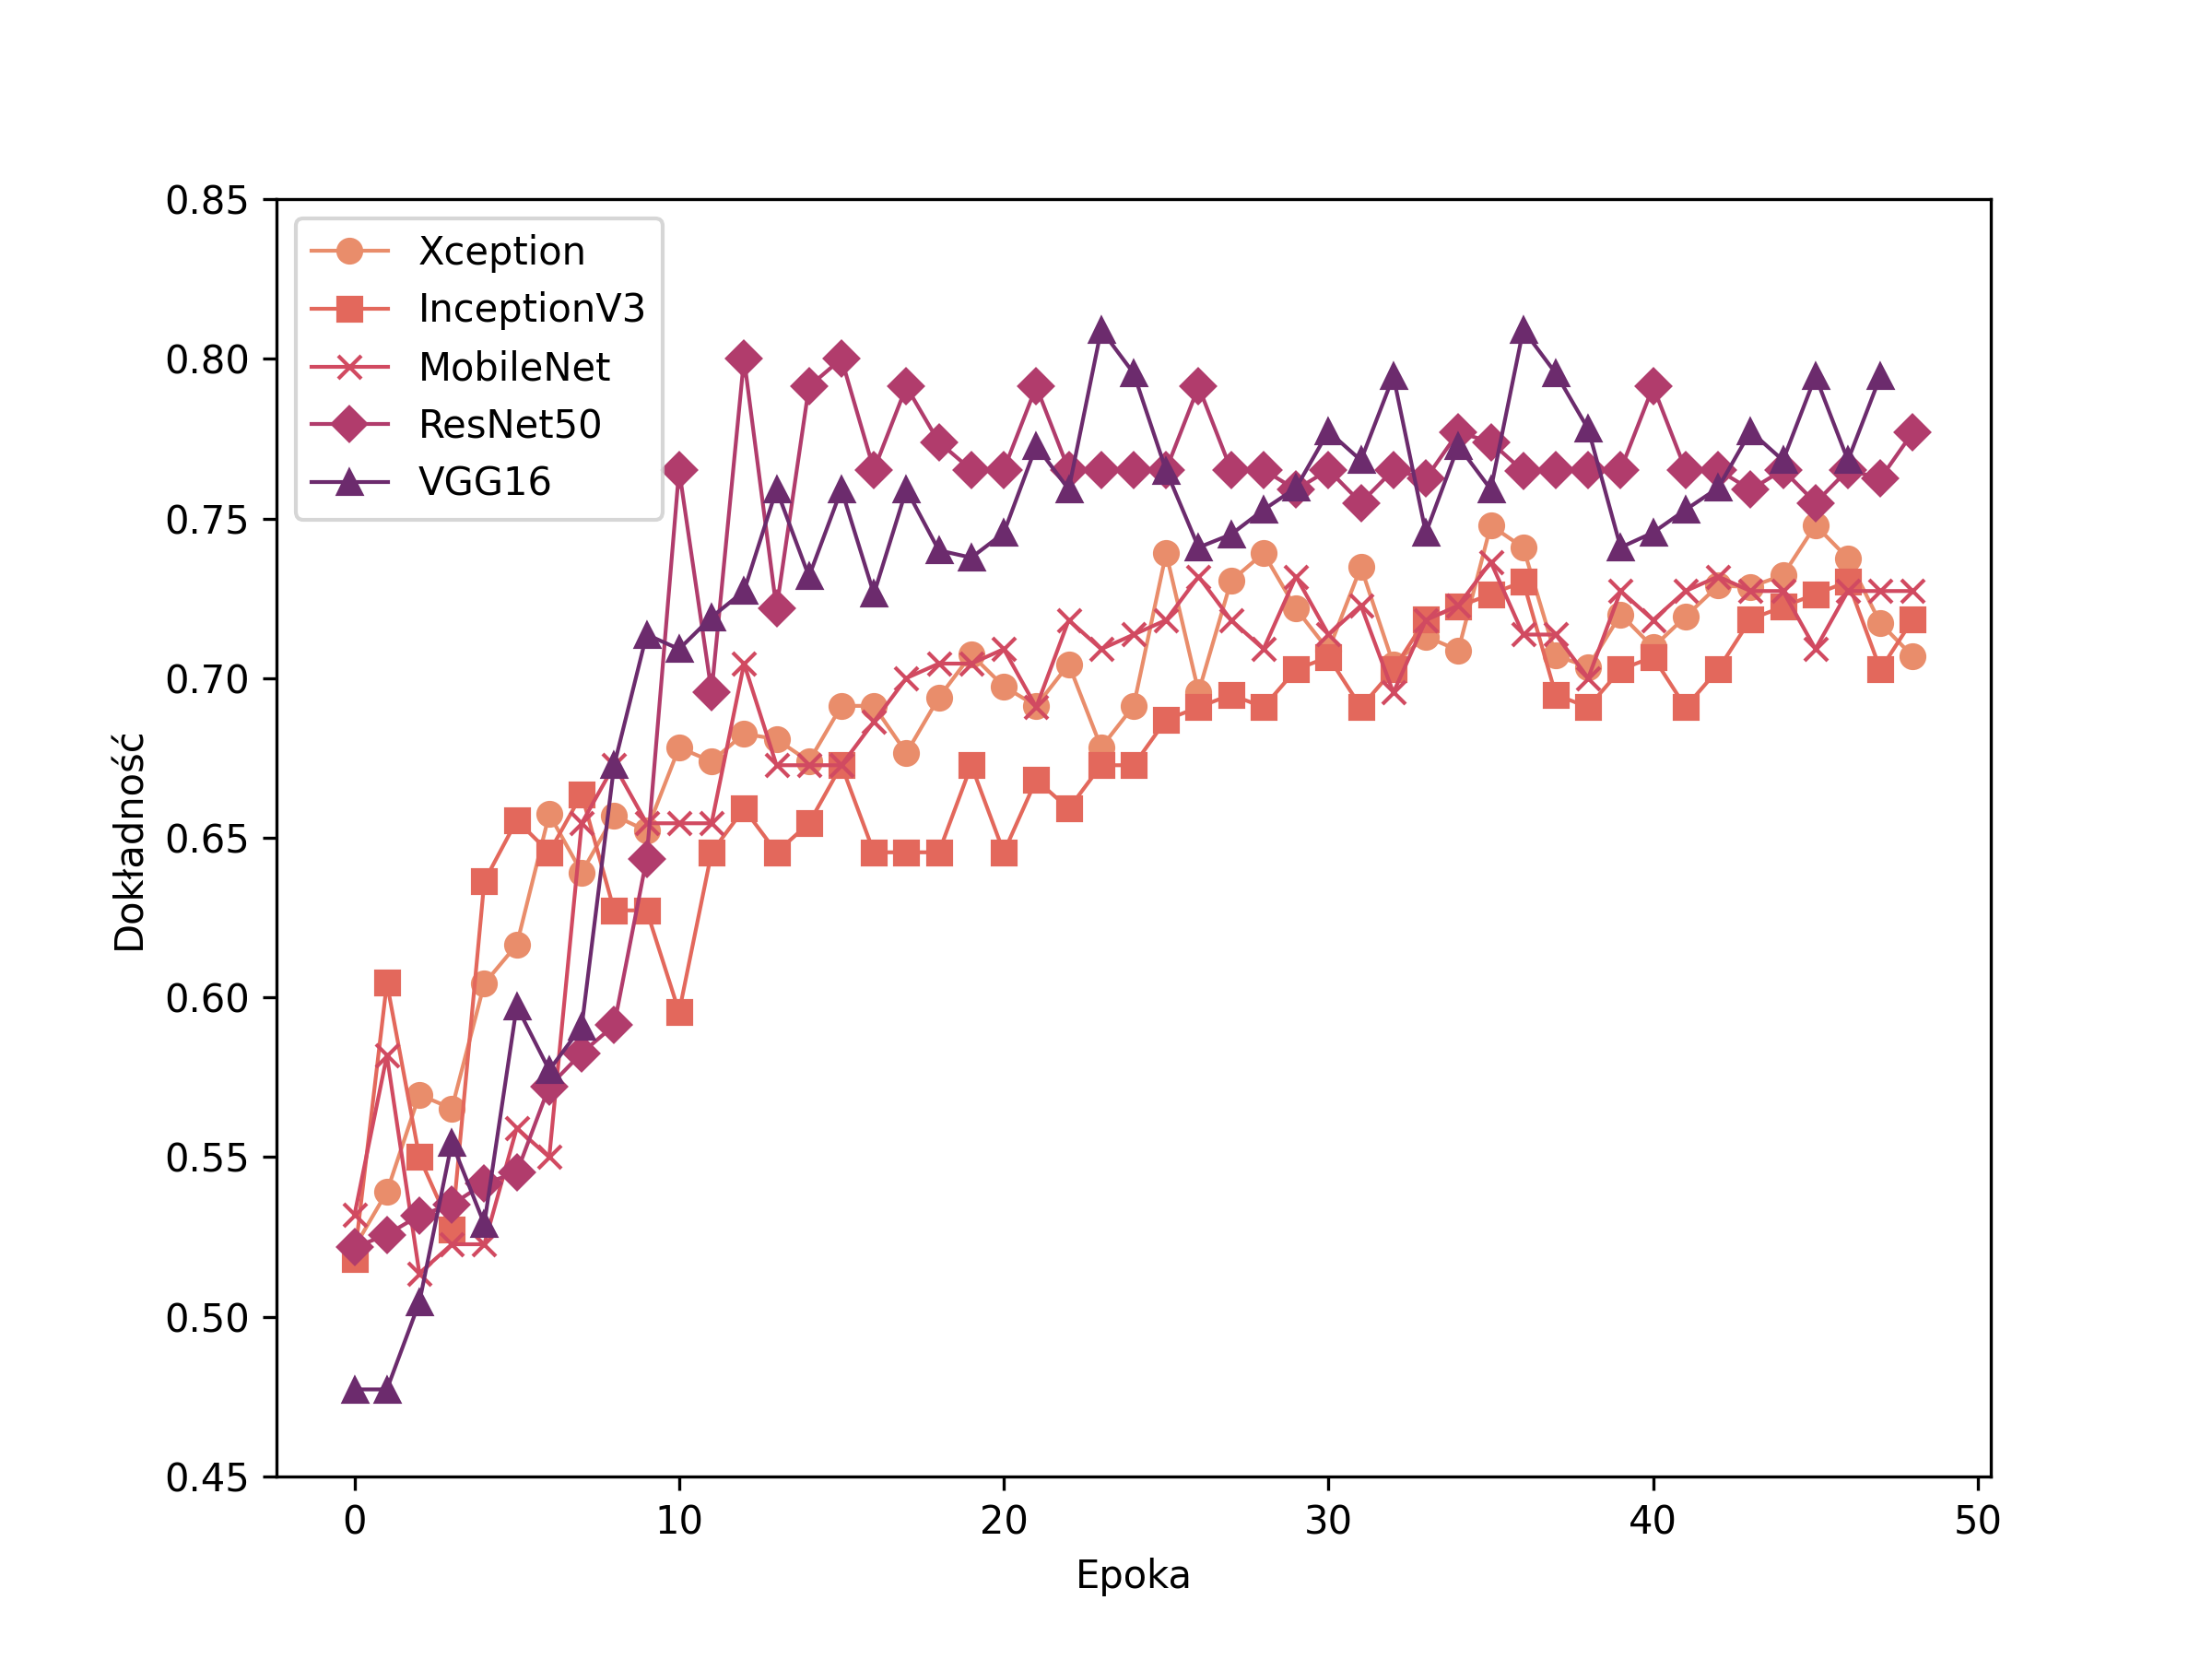
\includegraphics[width=\textwidth]{./img/results/a_acc}
        \caption{Krzywe dokładności na zbiorze walidacyjnym podczas uczenia\@}
        \label{fig:a_acc}
    \end{subfigure}
    \begin{subfigure}{0.49\textwidth}
        \centering
        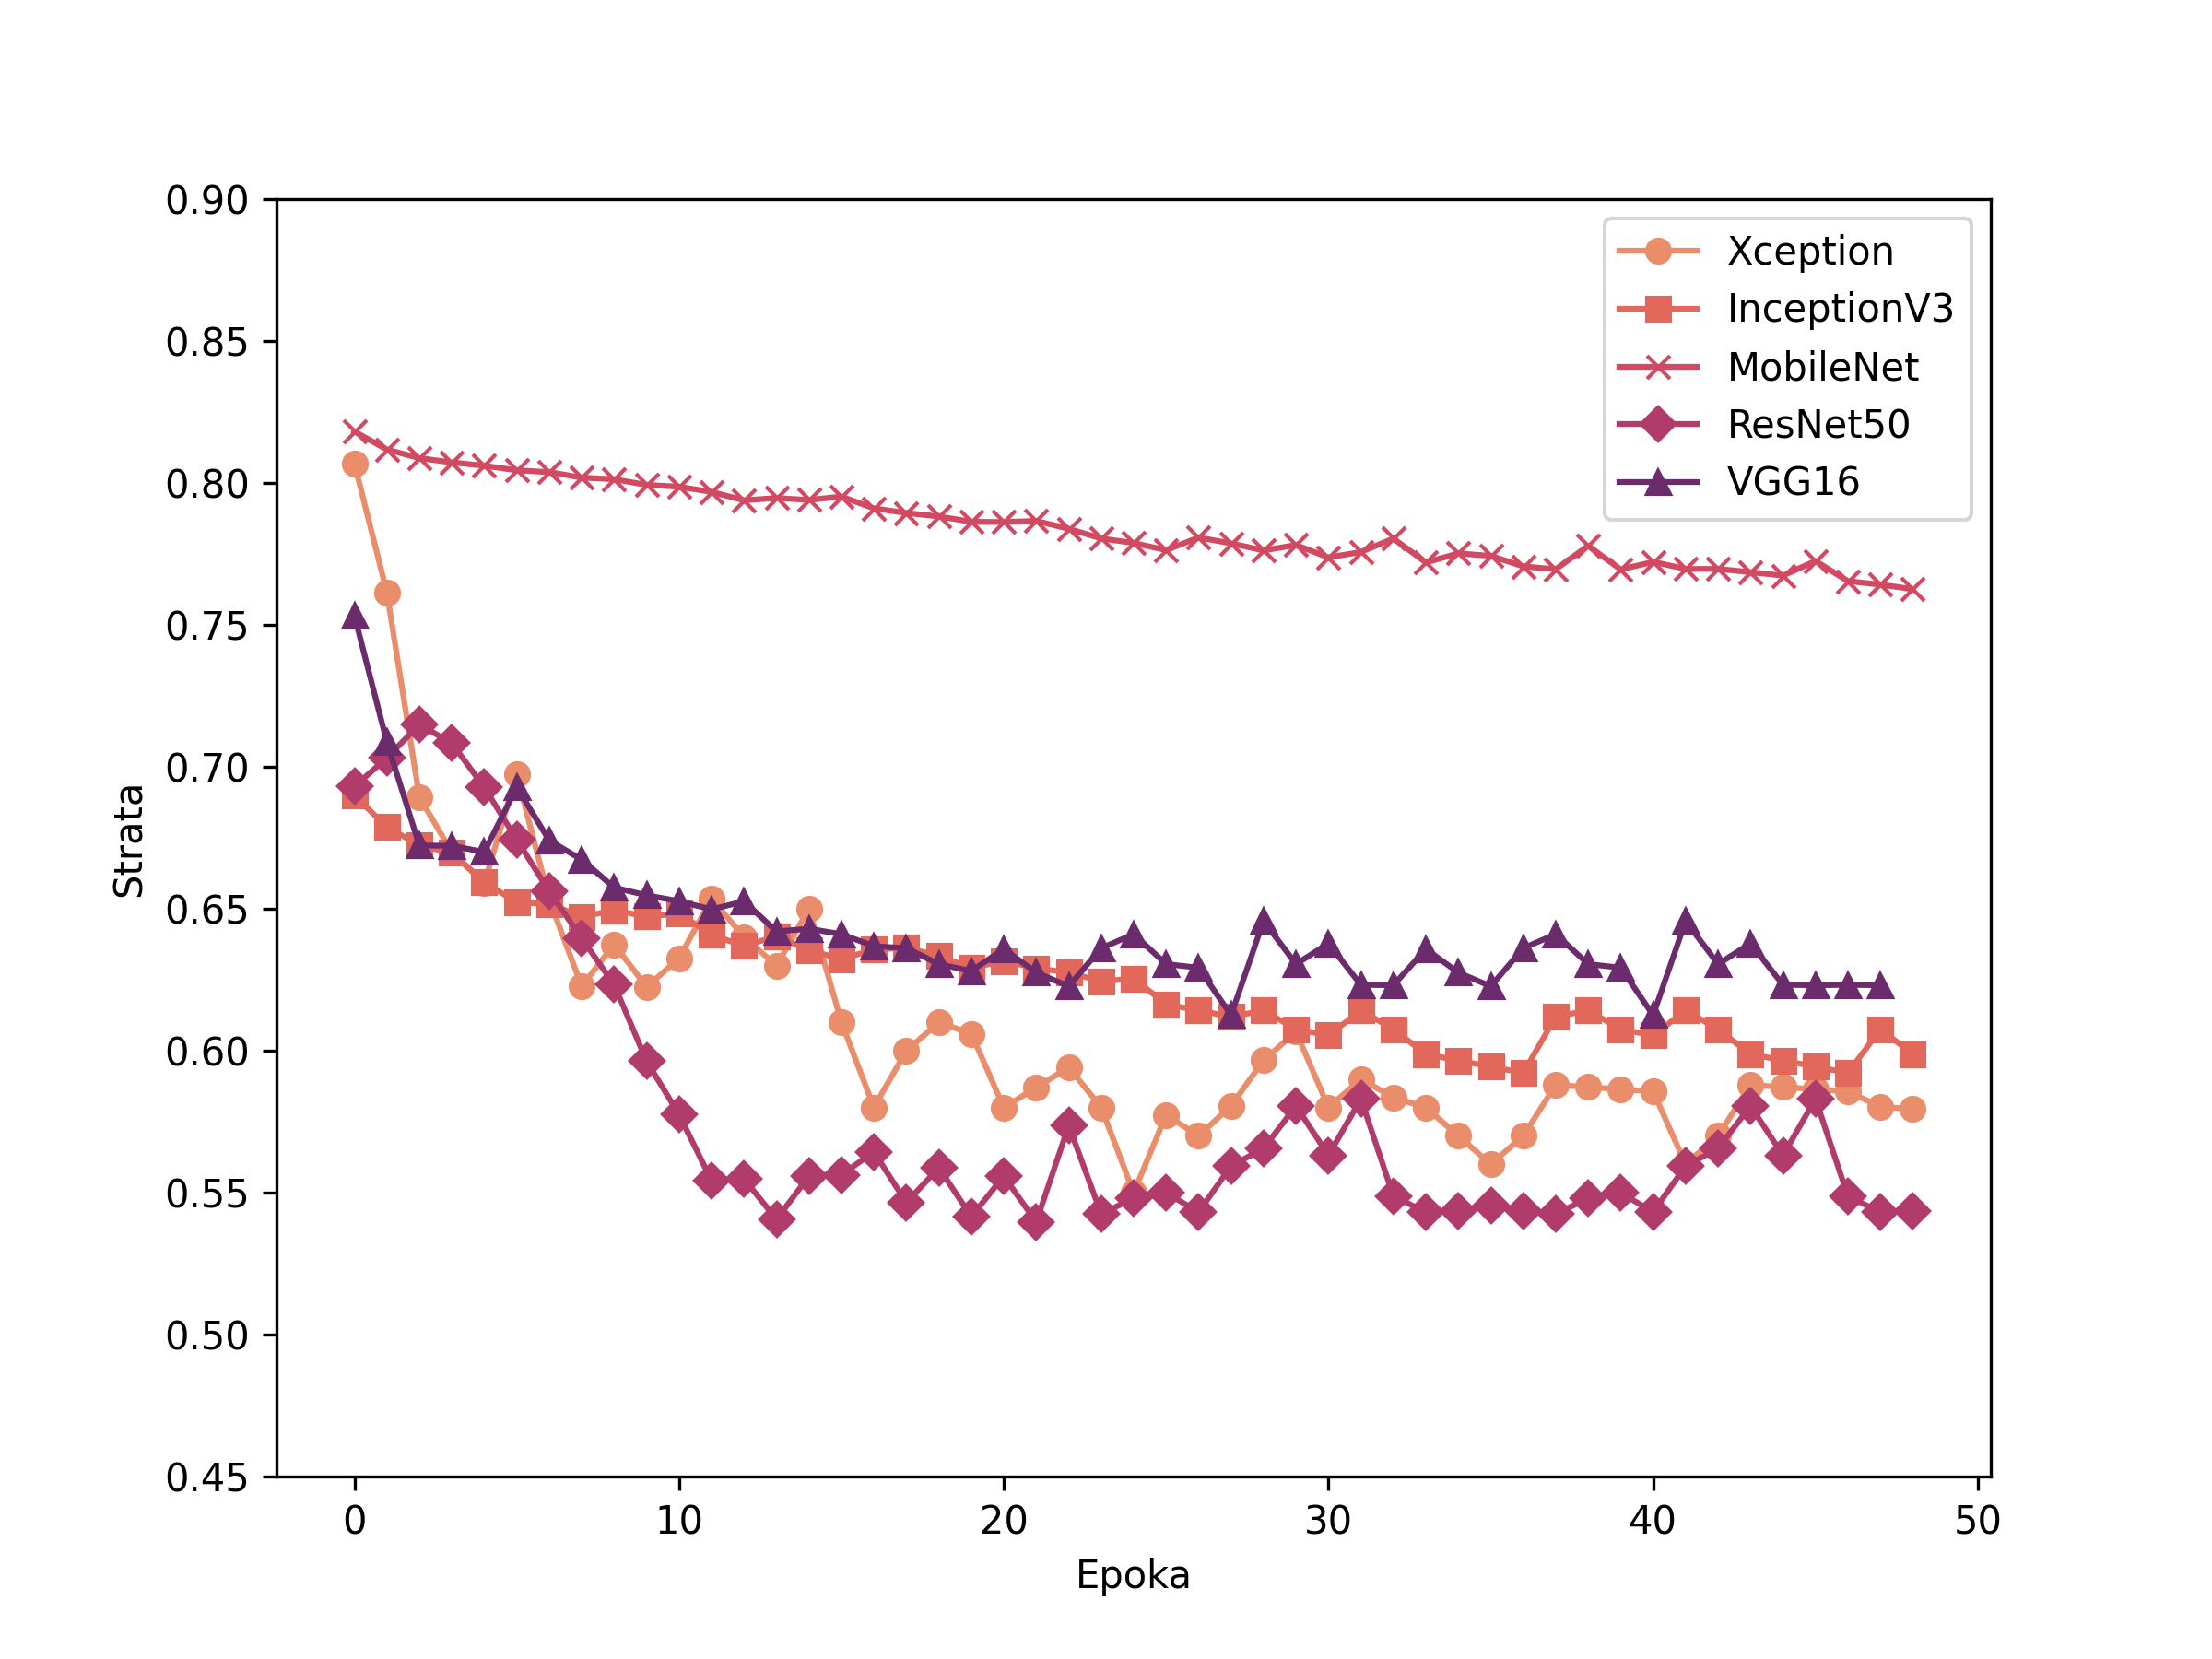
\includegraphics[width=\textwidth]{./img/results/a_loss}
        \caption{Krzywe funkcji straty na zbiorze walidacyjnym podczas uczenia\@}
        \label{fig:a_loss}
    \end{subfigure}

    \caption{Porównanie krzywych uczenia dla różnych klasyfikatorów na zbiorze walidacyjnym (samogłoska /a/)}
    \label{fig:a_results}
\end{figure}

%---------------------------------------------------------------------------

\section{Samogłoska /e/}
\label{sec:samogloska-e}

\begin{table}[h]
\centering
\caption{Wyniki otrzymane dla samogłoski /e/}
\label{tab:wyniki-e}
\begin{tabular}{|l|c|c|c|c|c|}
\hline
\textbf{Model} &\textbf{VGG16} &\textbf{Resnet50} &\textbf{Xception} &\textbf{InceptionV3} &\textbf{MobileNetV2} \\ \hline
    Accuracy &0.733 &0.621 &0.653 &0.644 &0.700 \\ \hline
    Precision &0.729 &0.625 &0.640 &0.641 &0.721 \\ \hline
    Recall &0.733 &0.620 &0.633 &0.638 &0.689 \\ \hline
    F1-score &0.735 &0.643 &0.649 &0.640 &0.692 \\ \hline
    Loss &0.582 &0.659 &0.632 &0.634 &0.601 \\ \hline
\end{tabular}
\end{table}


\begin{figure}[ht]
    \centering
    \begin{subfigure}{0.49\textwidth}
        \centering
        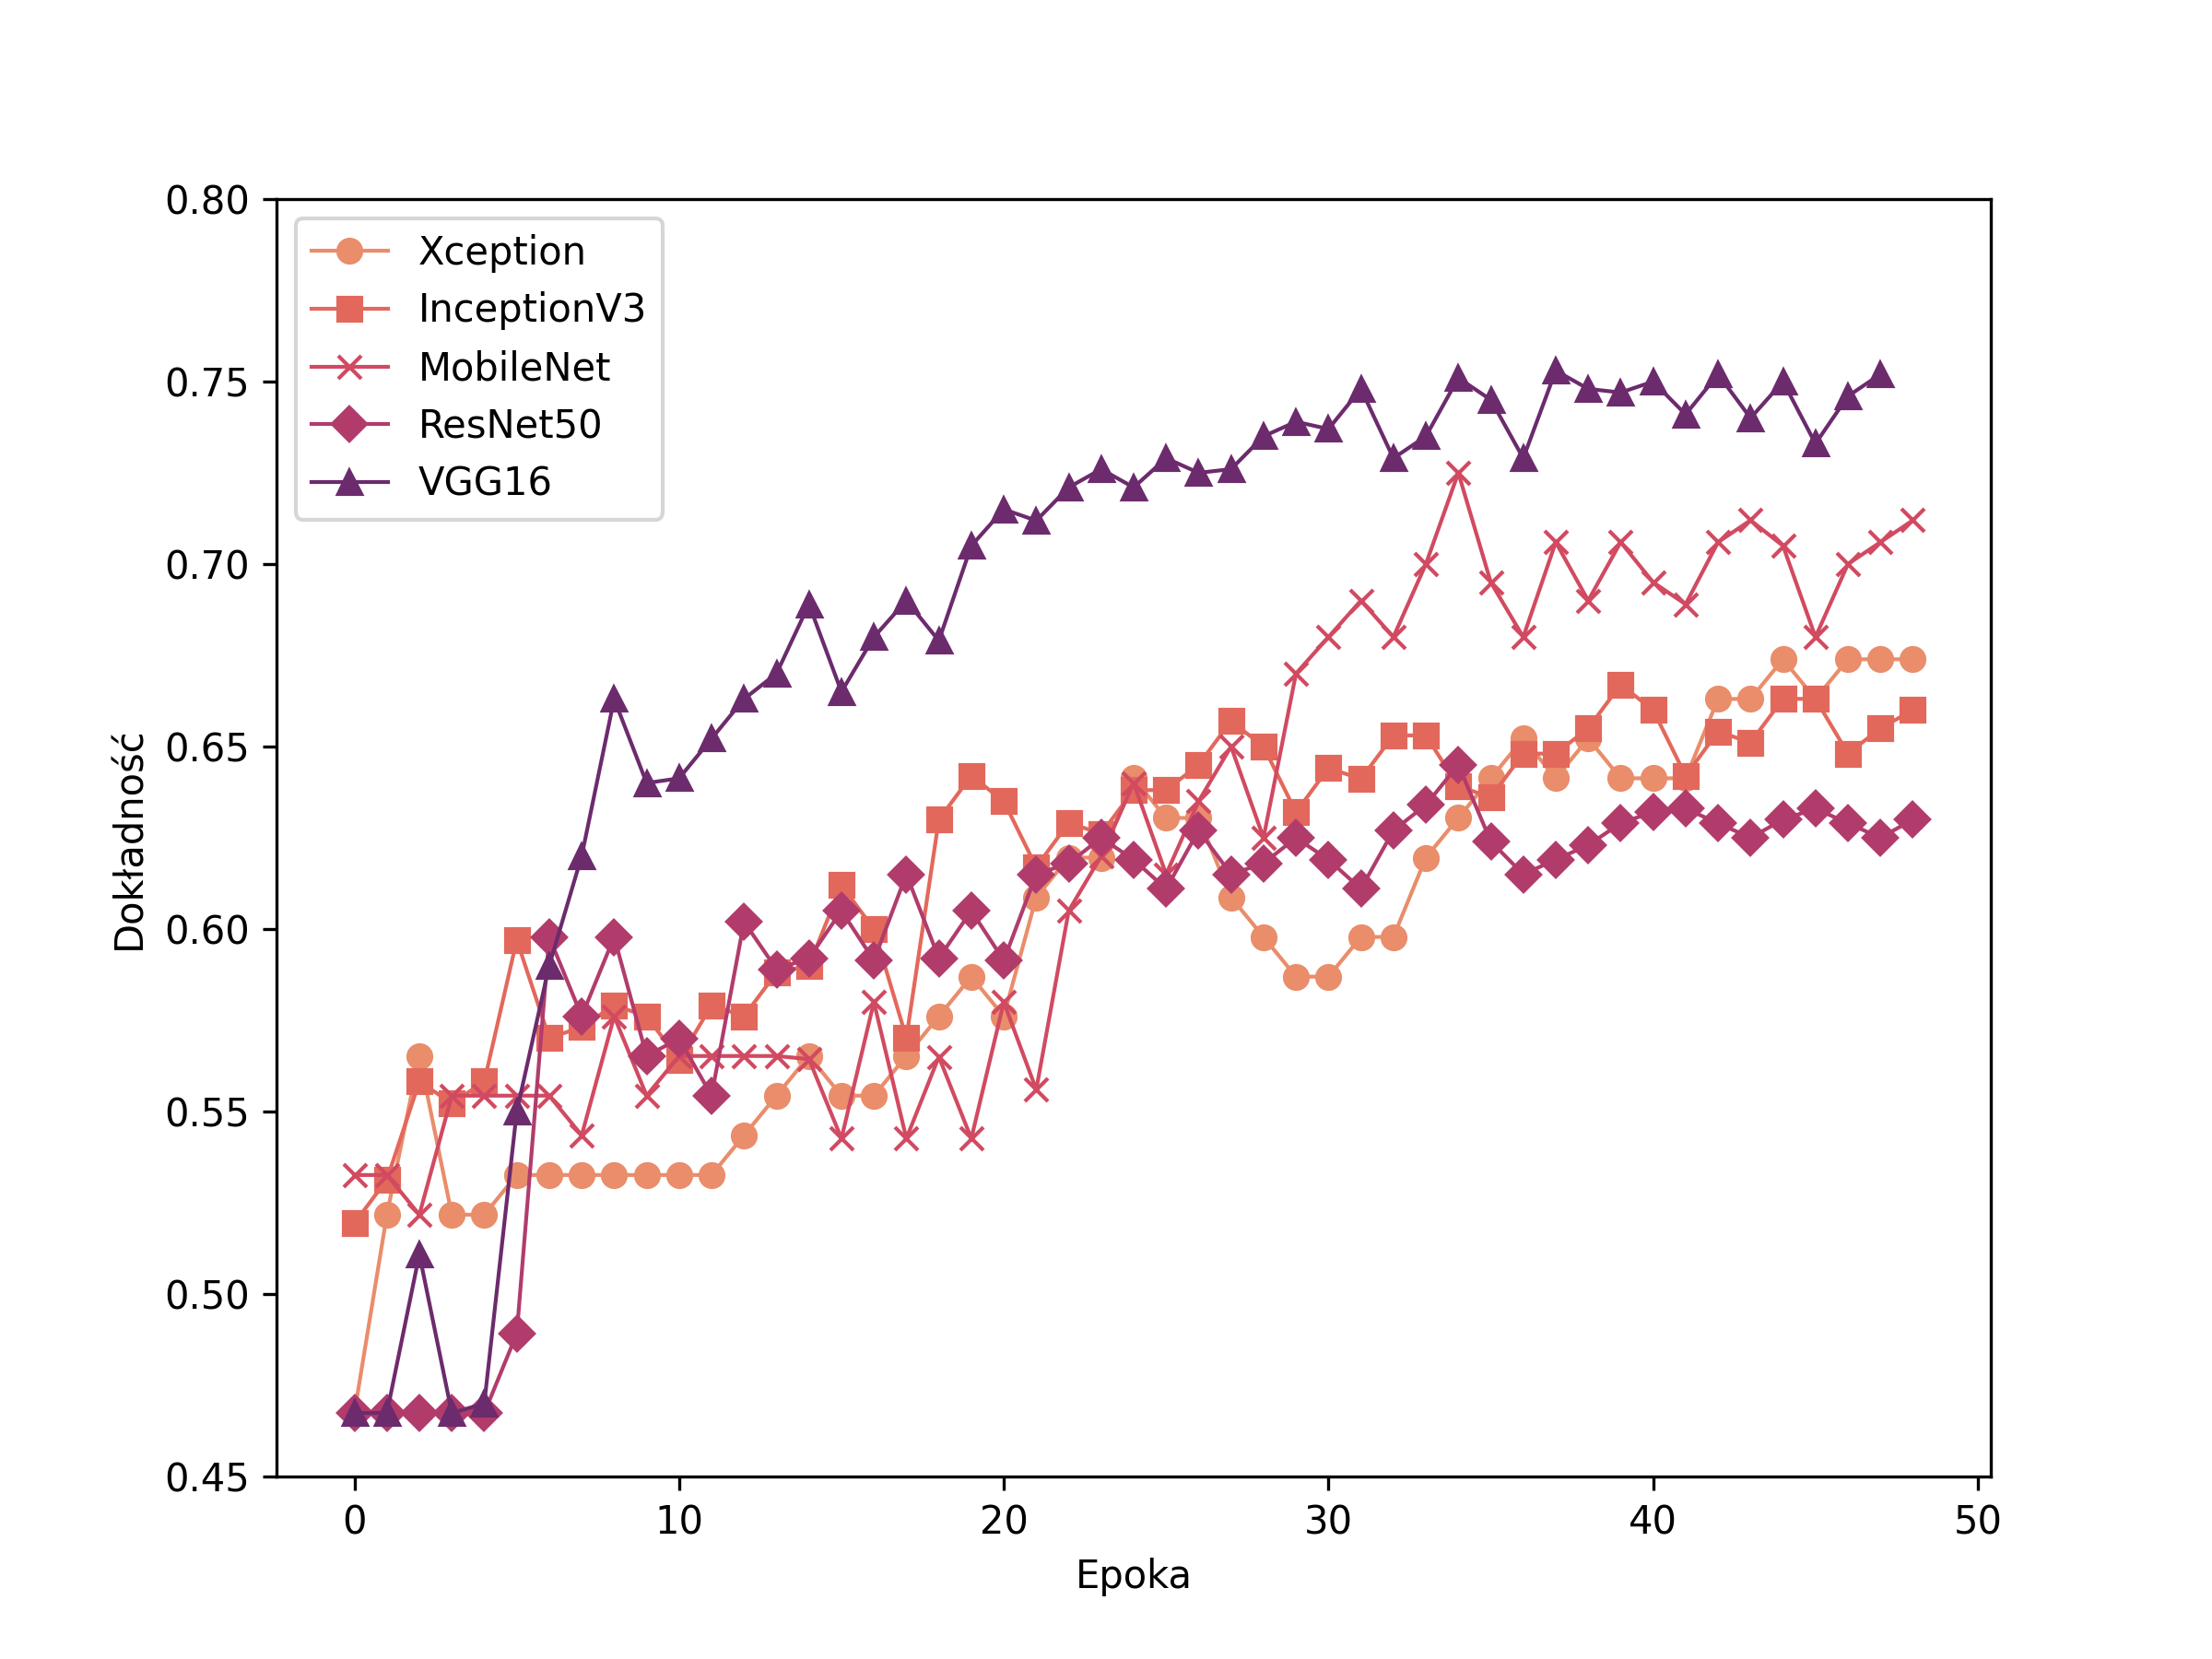
\includegraphics[width=\textwidth]{./img/results/e_acc}
        \caption{Krzywe dokładności na zbiorze walidacyjnym podczas uczenia\@}
        \label{fig:e_acc}
    \end{subfigure}
    \begin{subfigure}{0.49\textwidth}
        \centering
        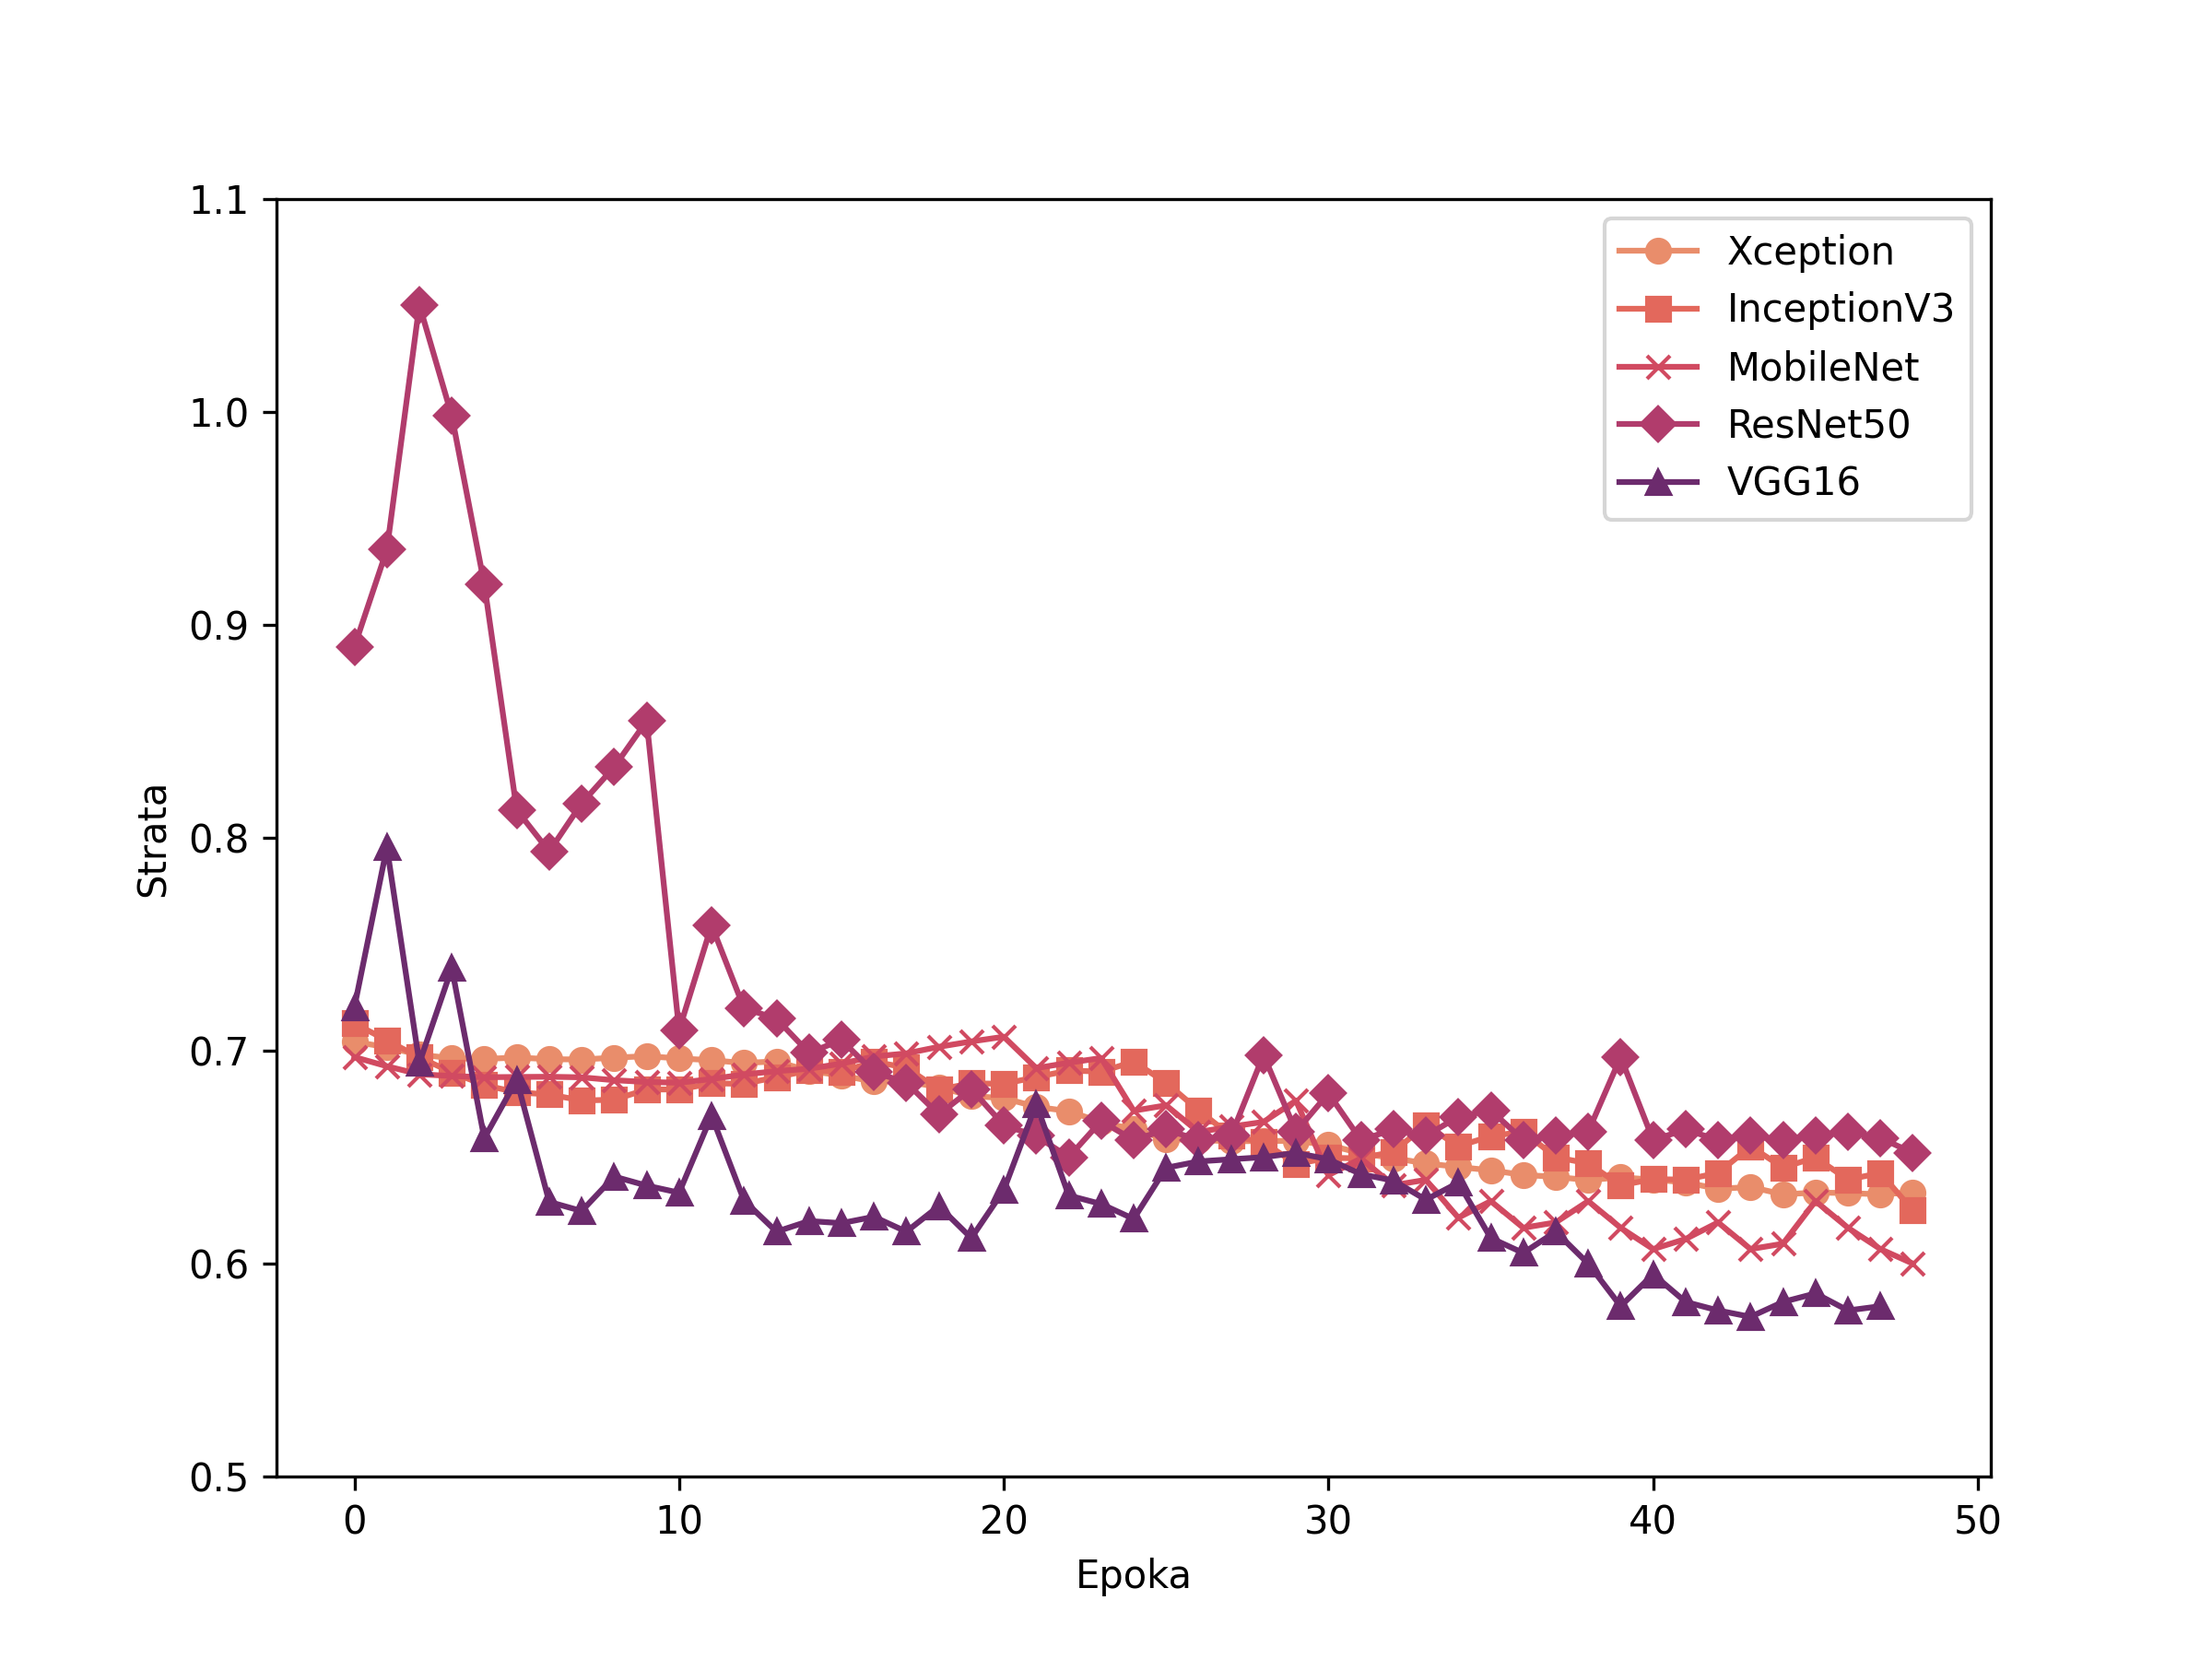
\includegraphics[width=\textwidth]{./img/results/e_loss}
        \caption{Krzywe funkcji straty na zbiorze walidacyjnym podczas uczenia\@}
        \label{fig:e_loss}
    \end{subfigure}

    \caption{Porównanie krzywych uczenia dla różnych klasyfikatorów na zbiorze walidacyjnym (samogłoska /e/)}
    \label{fig:e_results}
\end{figure}
%---------------------------------------------------------------------------

\section{Samogłoska /i/}
\label{sec:samogloska-i}

\begin{table}[h]
\centering
\caption{Wyniki otrzymane dla samogłoski /i/}
\label{tab:wyniki-i}
\begin{tabular}{|l|c|c|c|c|c|}
\hline
\textbf{Model} &\textbf{VGG16} &\textbf{Resnet50} &\textbf{Xception} &\textbf{InceptionV3} &\textbf{MobileNetV2} \\ \hline
    Accuracy &0.627 &0.586 &0.641 &0.605 &0.634 \\ \hline
    Precision &0.642 &0.589 &0.638 &0.598 &0.672 \\ \hline
    Recall &0.616 &0.584 &0.642 &0.595  &0.623 \\ \hline
    F1-score &0.0.605 &0.572 &0.643 &0.597 &0.614 \\ \hline
    Loss &0.775 &0.699 &0.751 &0.686 &0.656 \\ \hline
\end{tabular}
\end{table}

\begin{figure}[ht]
    \centering
    \begin{subfigure}{0.49\textwidth}
        \centering
        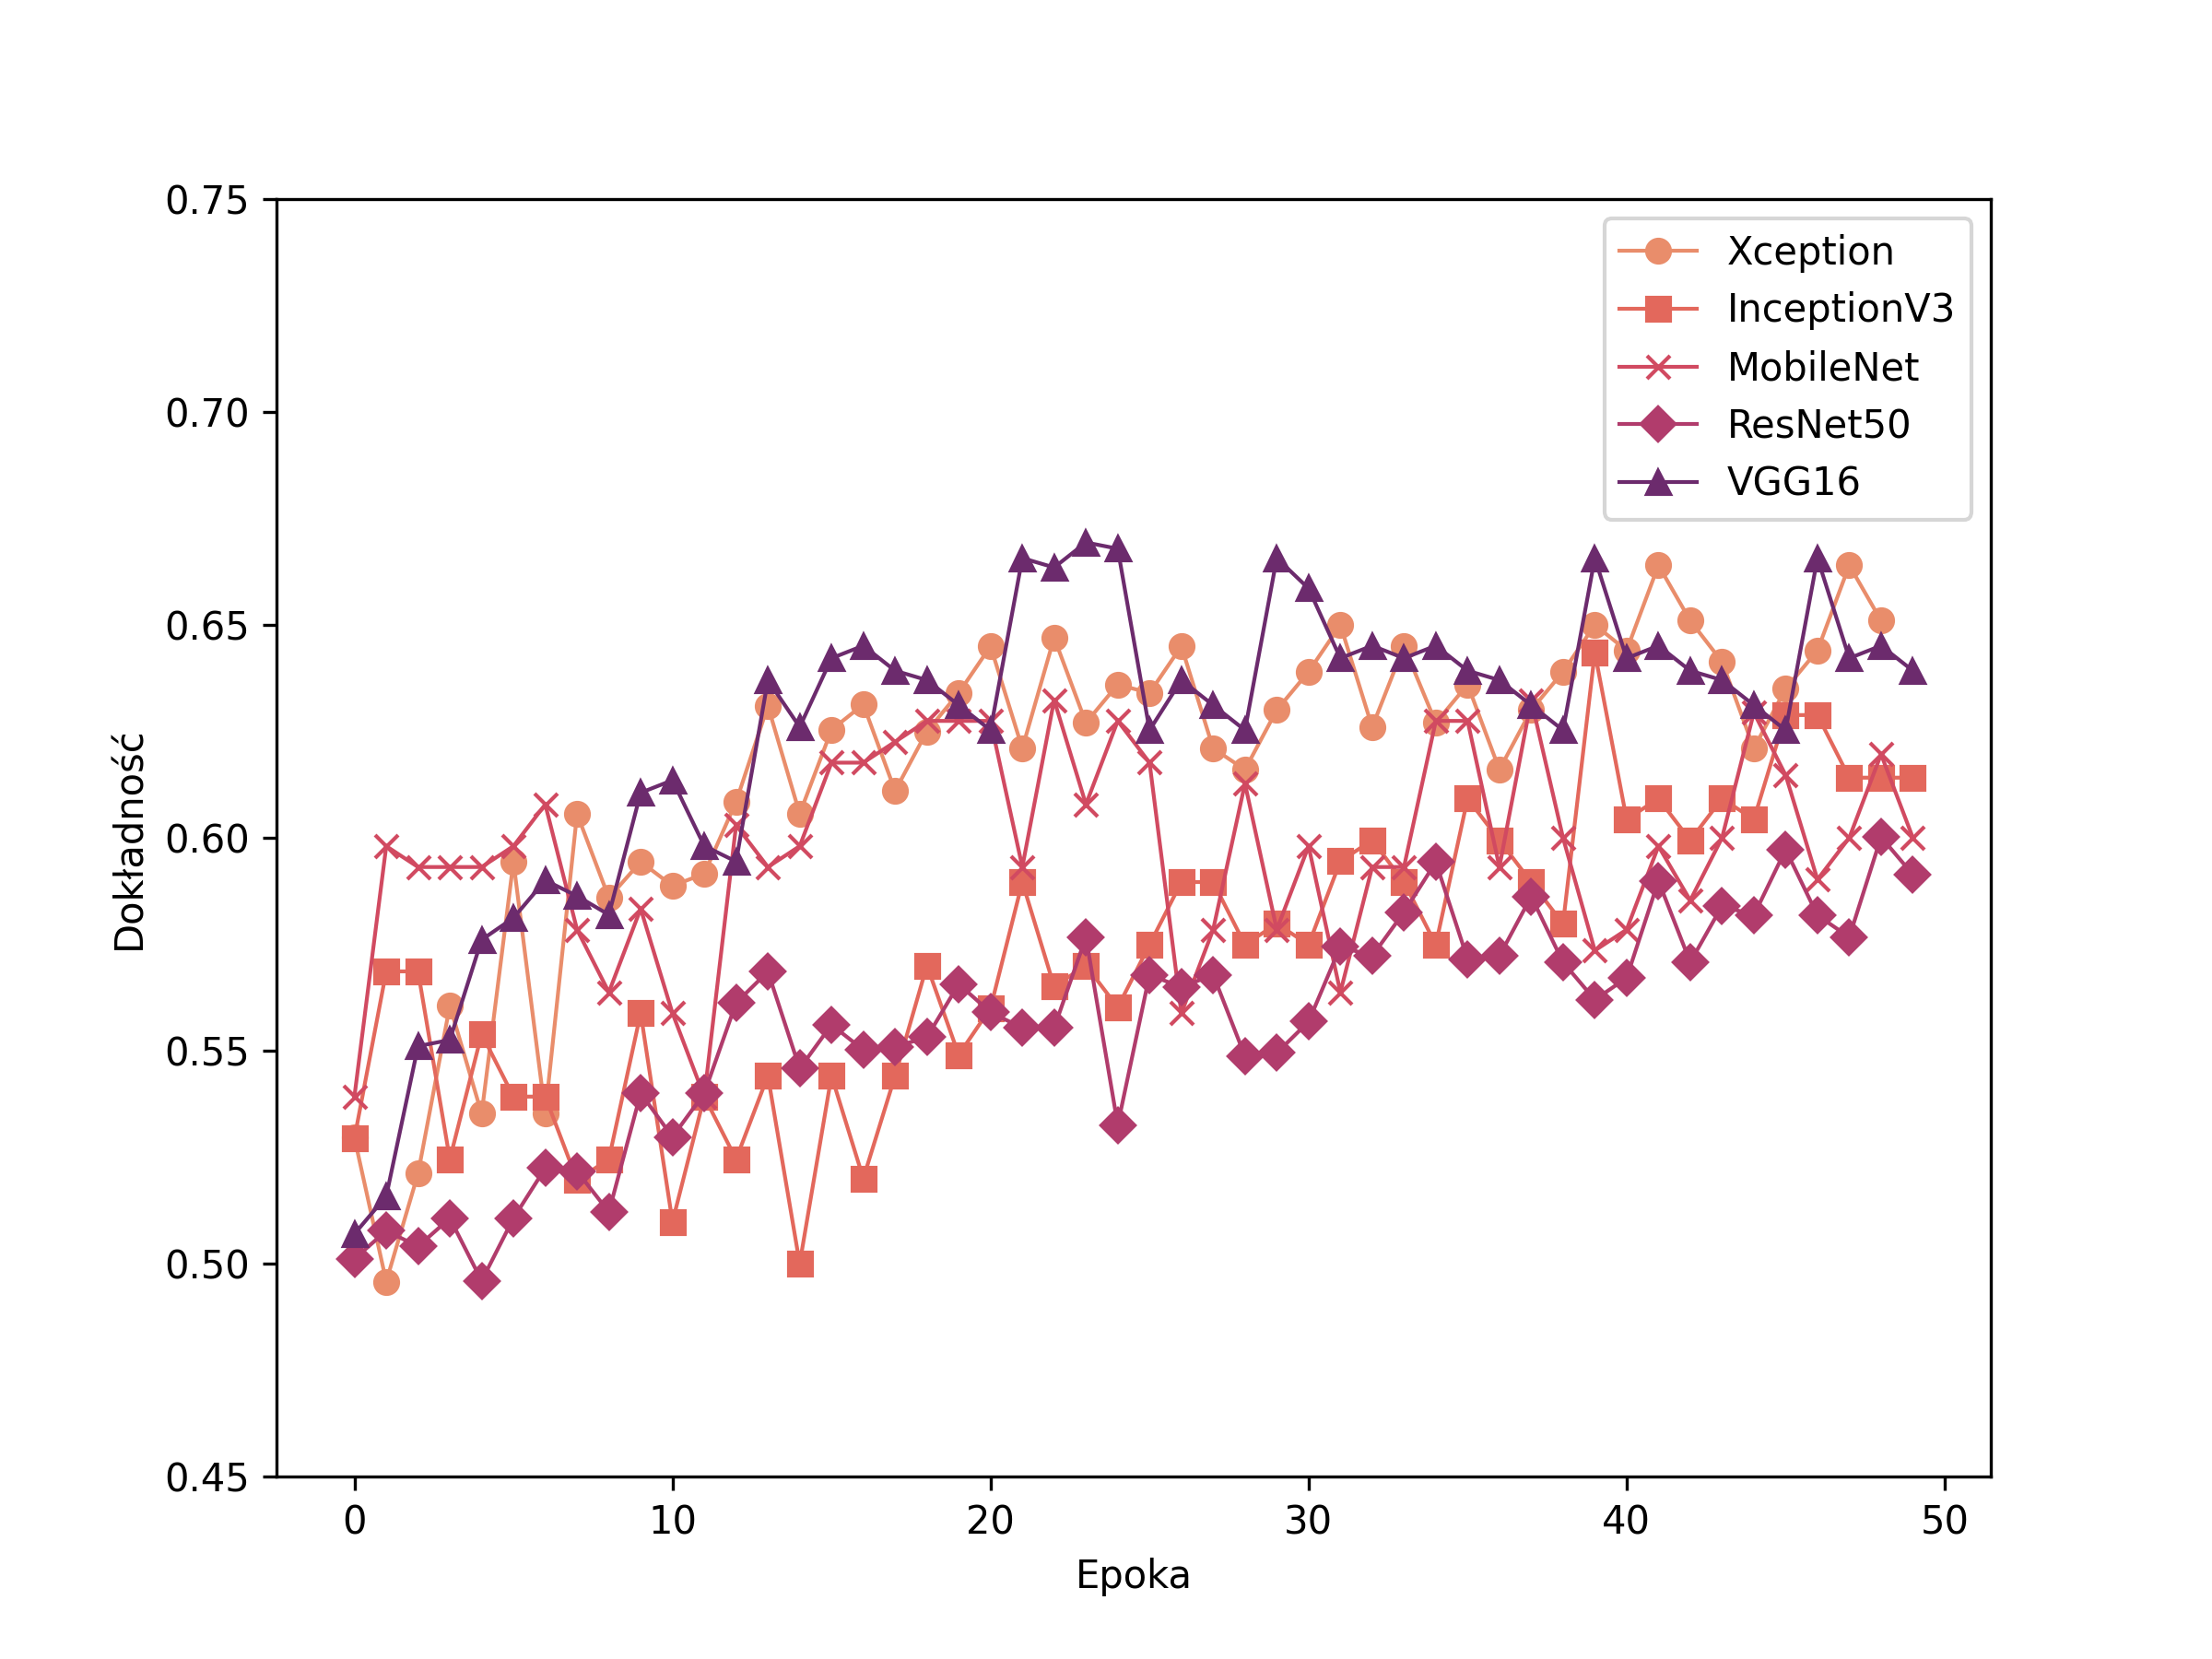
\includegraphics[width=\textwidth]{./img/results/i_acc}
        \caption{Krzywe dokładności na zbiorze walidacyjnym podczas uczenia\@}
        \label{fig:i_acc}
    \end{subfigure}
    \begin{subfigure}{0.49\textwidth}
        \centering
        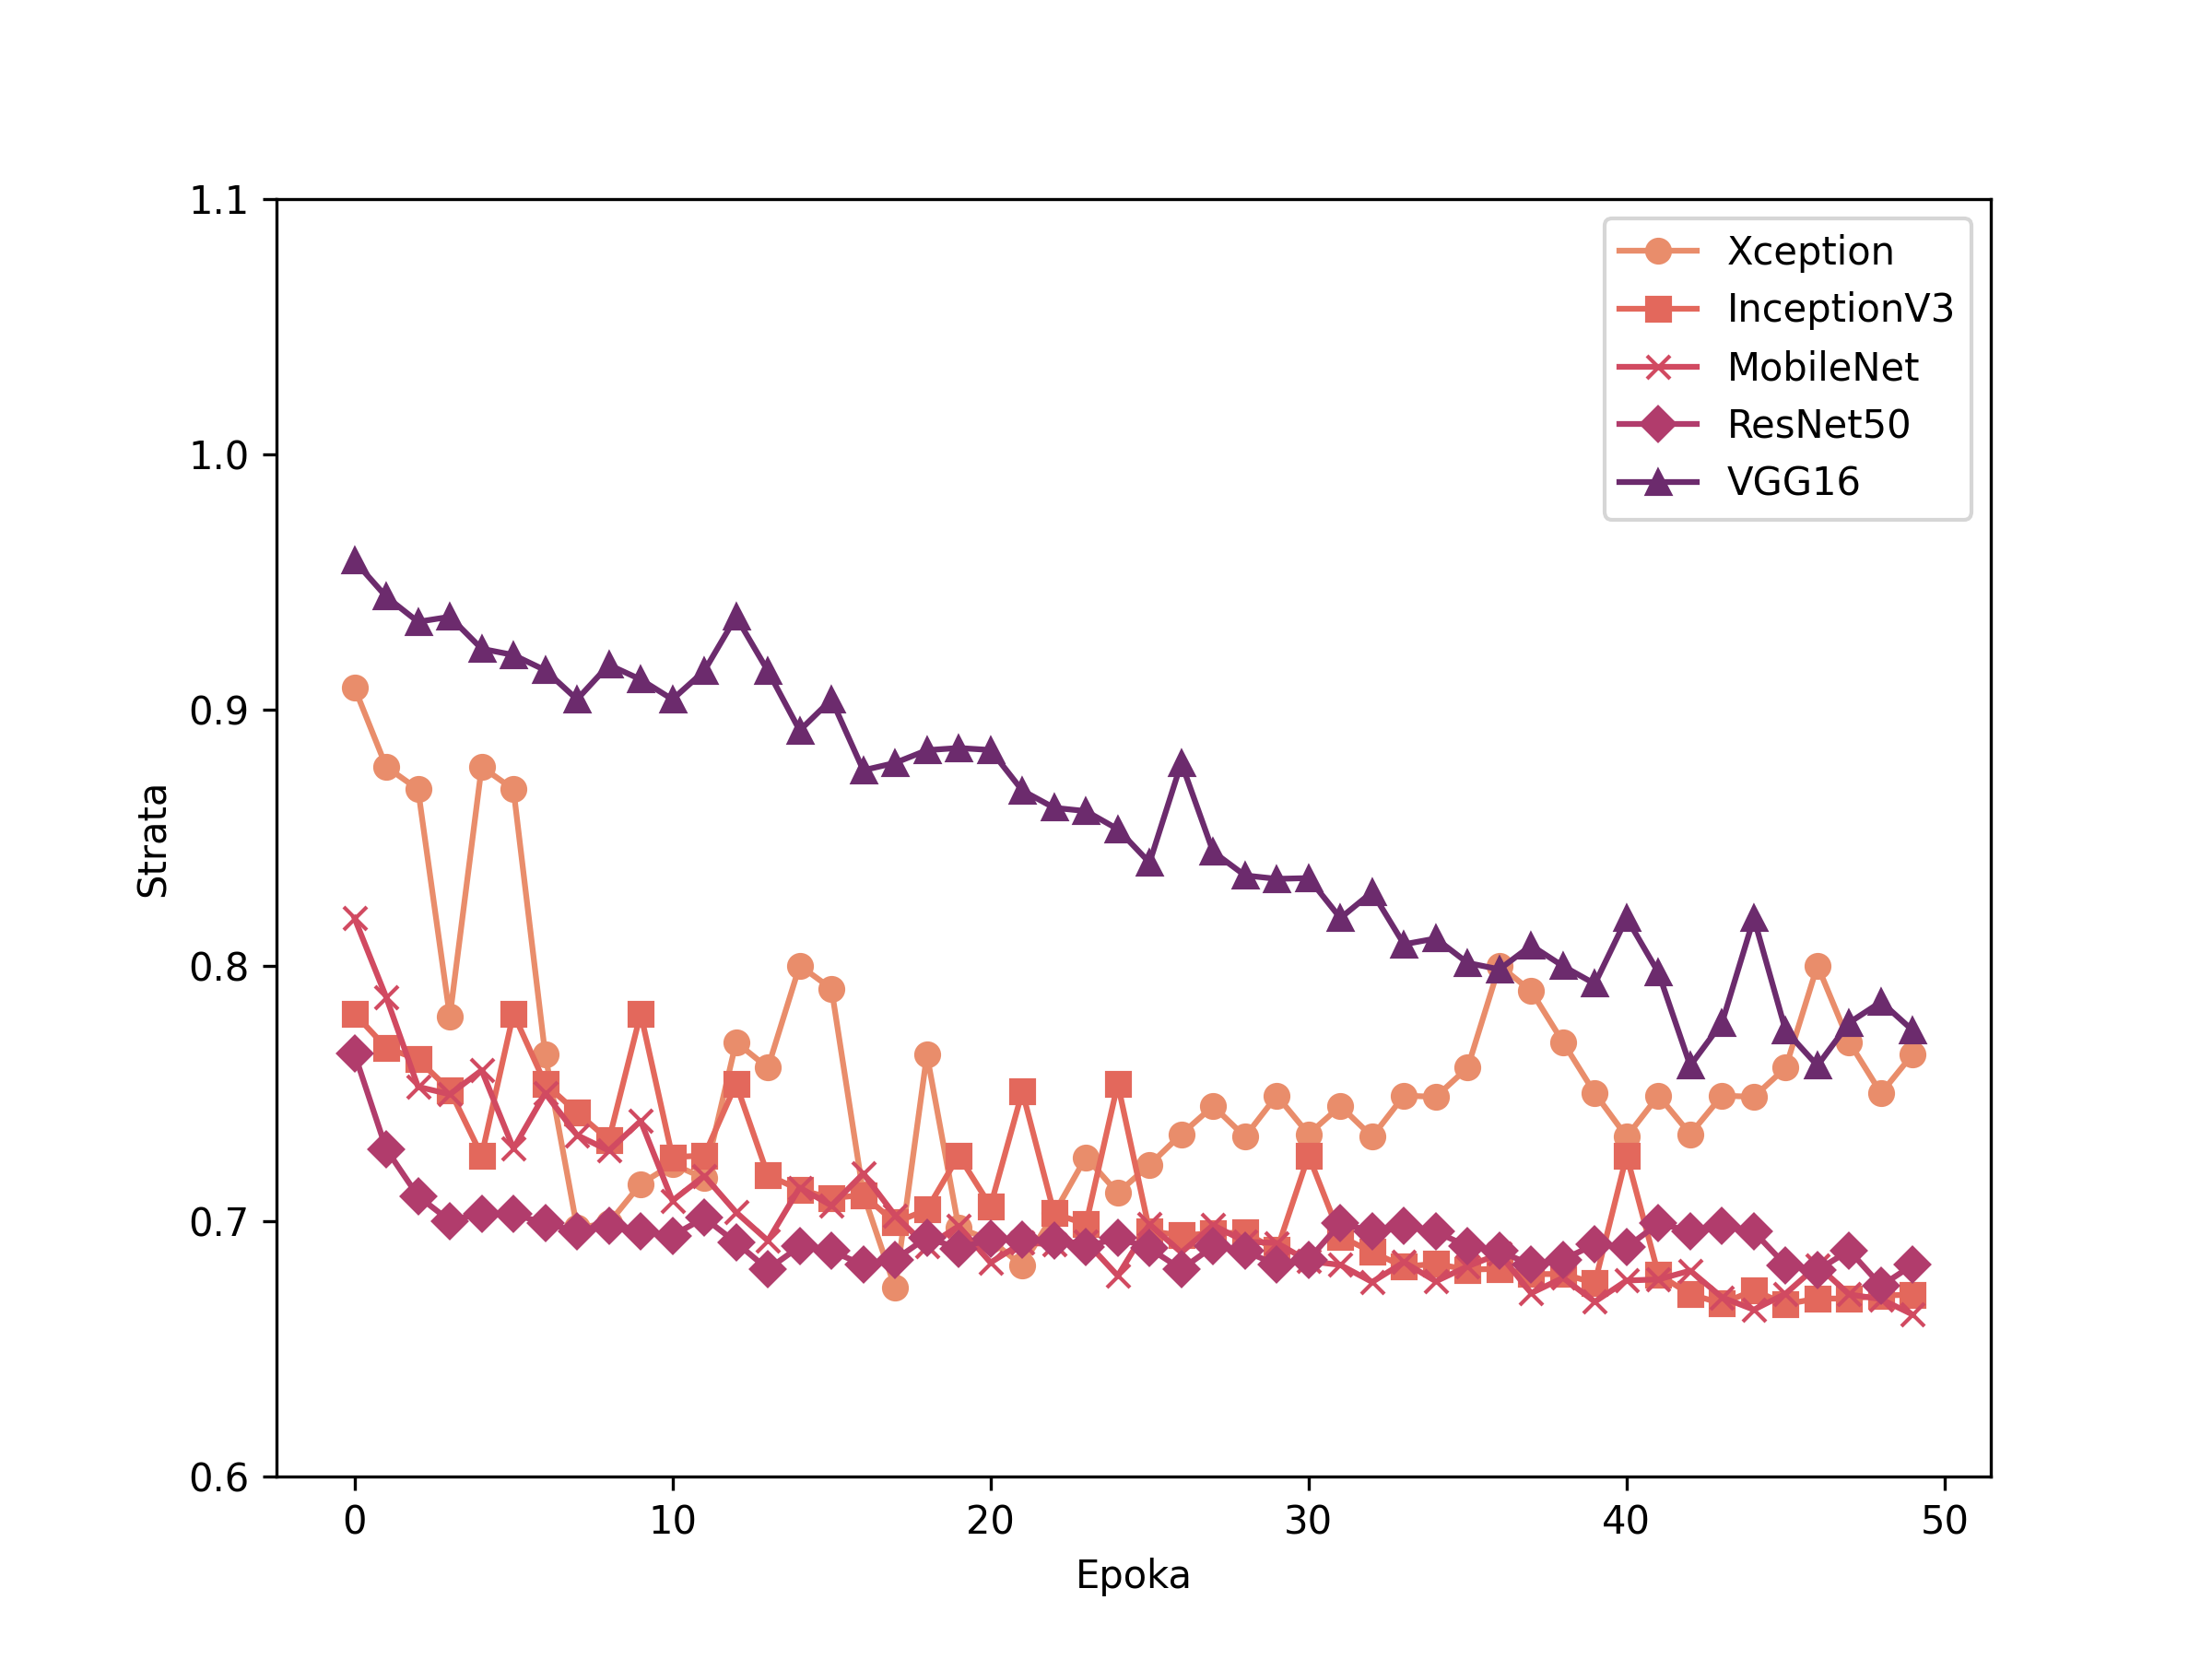
\includegraphics[width=\textwidth]{./img/results/i_loss}
        \caption{Krzywe funkcji straty na zbiorze walidacyjnym podczas uczenia\@}
        \label{fig:i_loss}
    \end{subfigure}

    \caption{Porównanie krzywych uczenia dla różnych klasyfikatorów na zbiorze walidacyjnym (samogłoska /i/)}
    \label{fig:i_results}
\end{figure}

%---------------------------------------------------------------------------

\section{Samogłoska /o/}
\label{sec:samogloska-o}

\begin{table}[h]
\centering
\caption{Wyniki otrzymane dla samogłoski /o/}
\label{tab:wyniki-o}
\begin{tabular}{|l|c|c|c|c|c|}
\hline
\textbf{Model} &\textbf{VGG16} &\textbf{Resnet50} &\textbf{Xception} &\textbf{InceptionV3} &\textbf{MobileNetV2} \\ \hline
    Accuracy &0.653 &0.632 &0.653 &0.611 &0.611 \\ \hline
    Precision &0.654 &0.651 &0.651 &0.612 &0.624 \\ \hline
    Recall &0.649 &0.635 &0.649 &0.609 &0.606 \\ \hline
    F1-score &0.650 &0.633 &0.646 &0.601 &0.594 \\ \hline
    Loss &0.674 &0.679 &0.662 &0.679 &0.677 \\ \hline
\end{tabular}
\end{table}

\begin{figure}[ht]
    \centering
    \begin{subfigure}{0.49\textwidth}
        \centering
        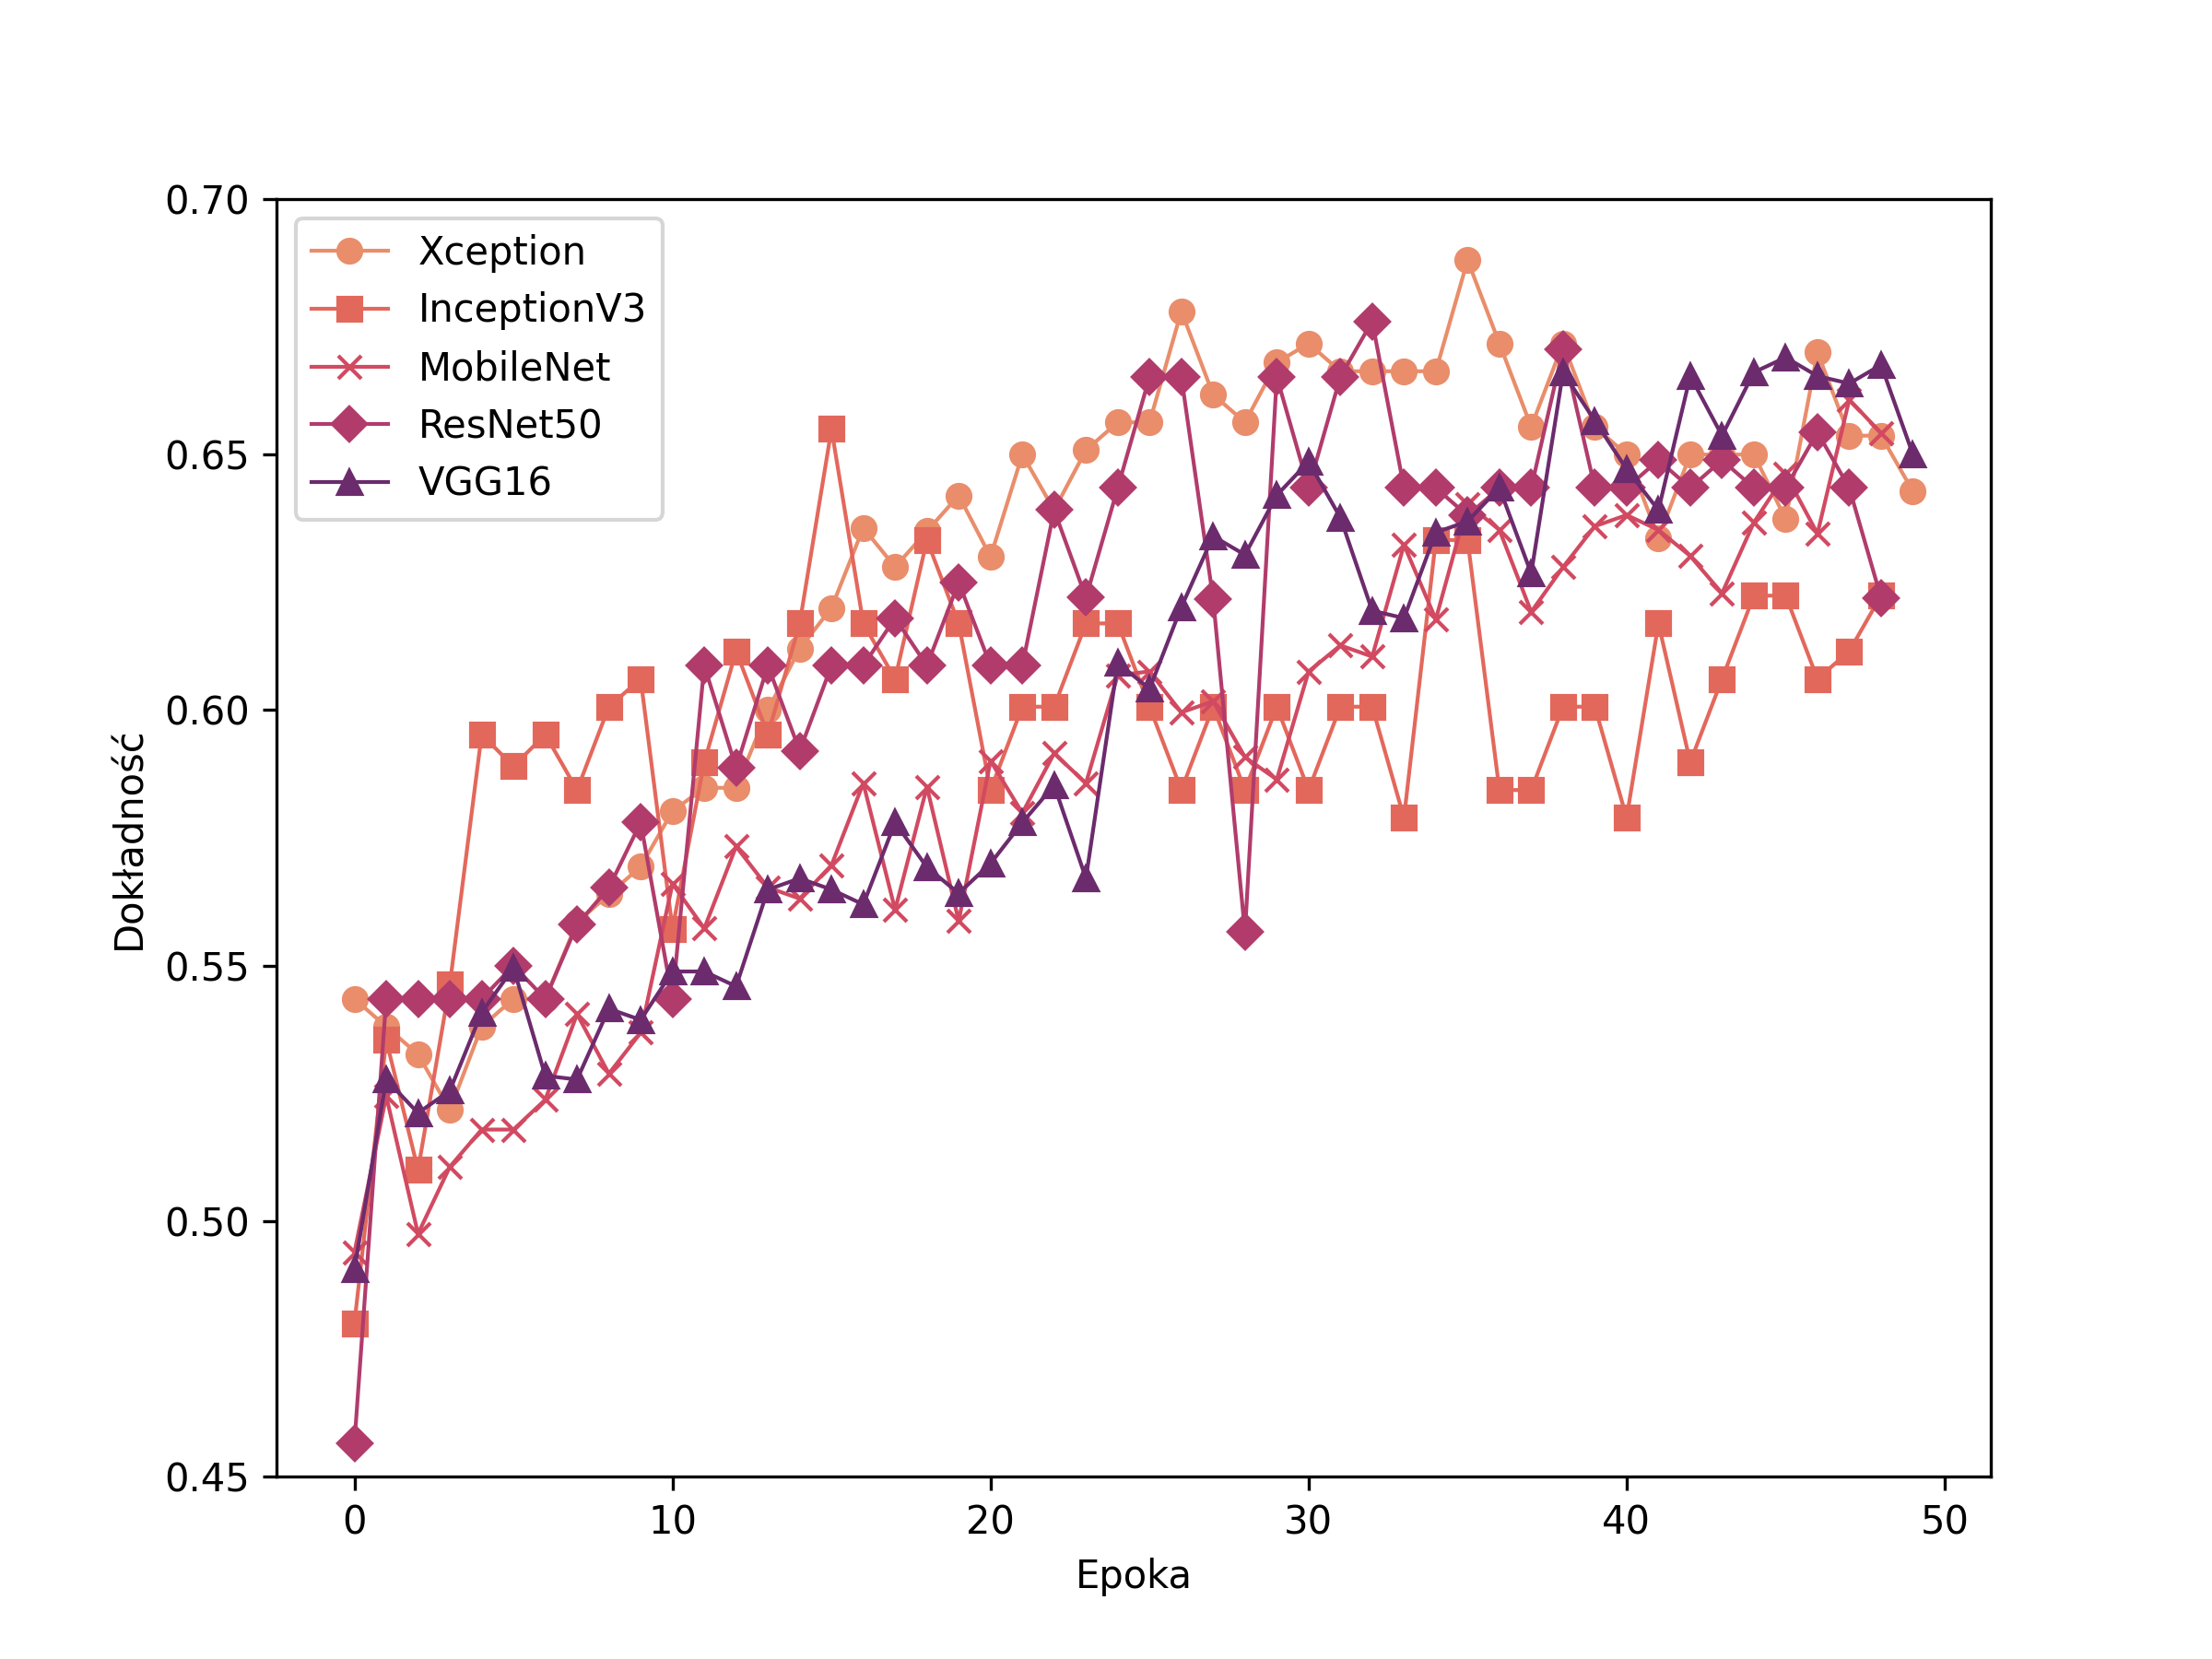
\includegraphics[width=\textwidth]{./img/results/o_acc}
        \caption{Krzywe dokładności na zbiorze walidacyjnym podczas uczenia\@}
        \label{fig:o_acc}
    \end{subfigure}
    \begin{subfigure}{0.49\textwidth}
        \centering
        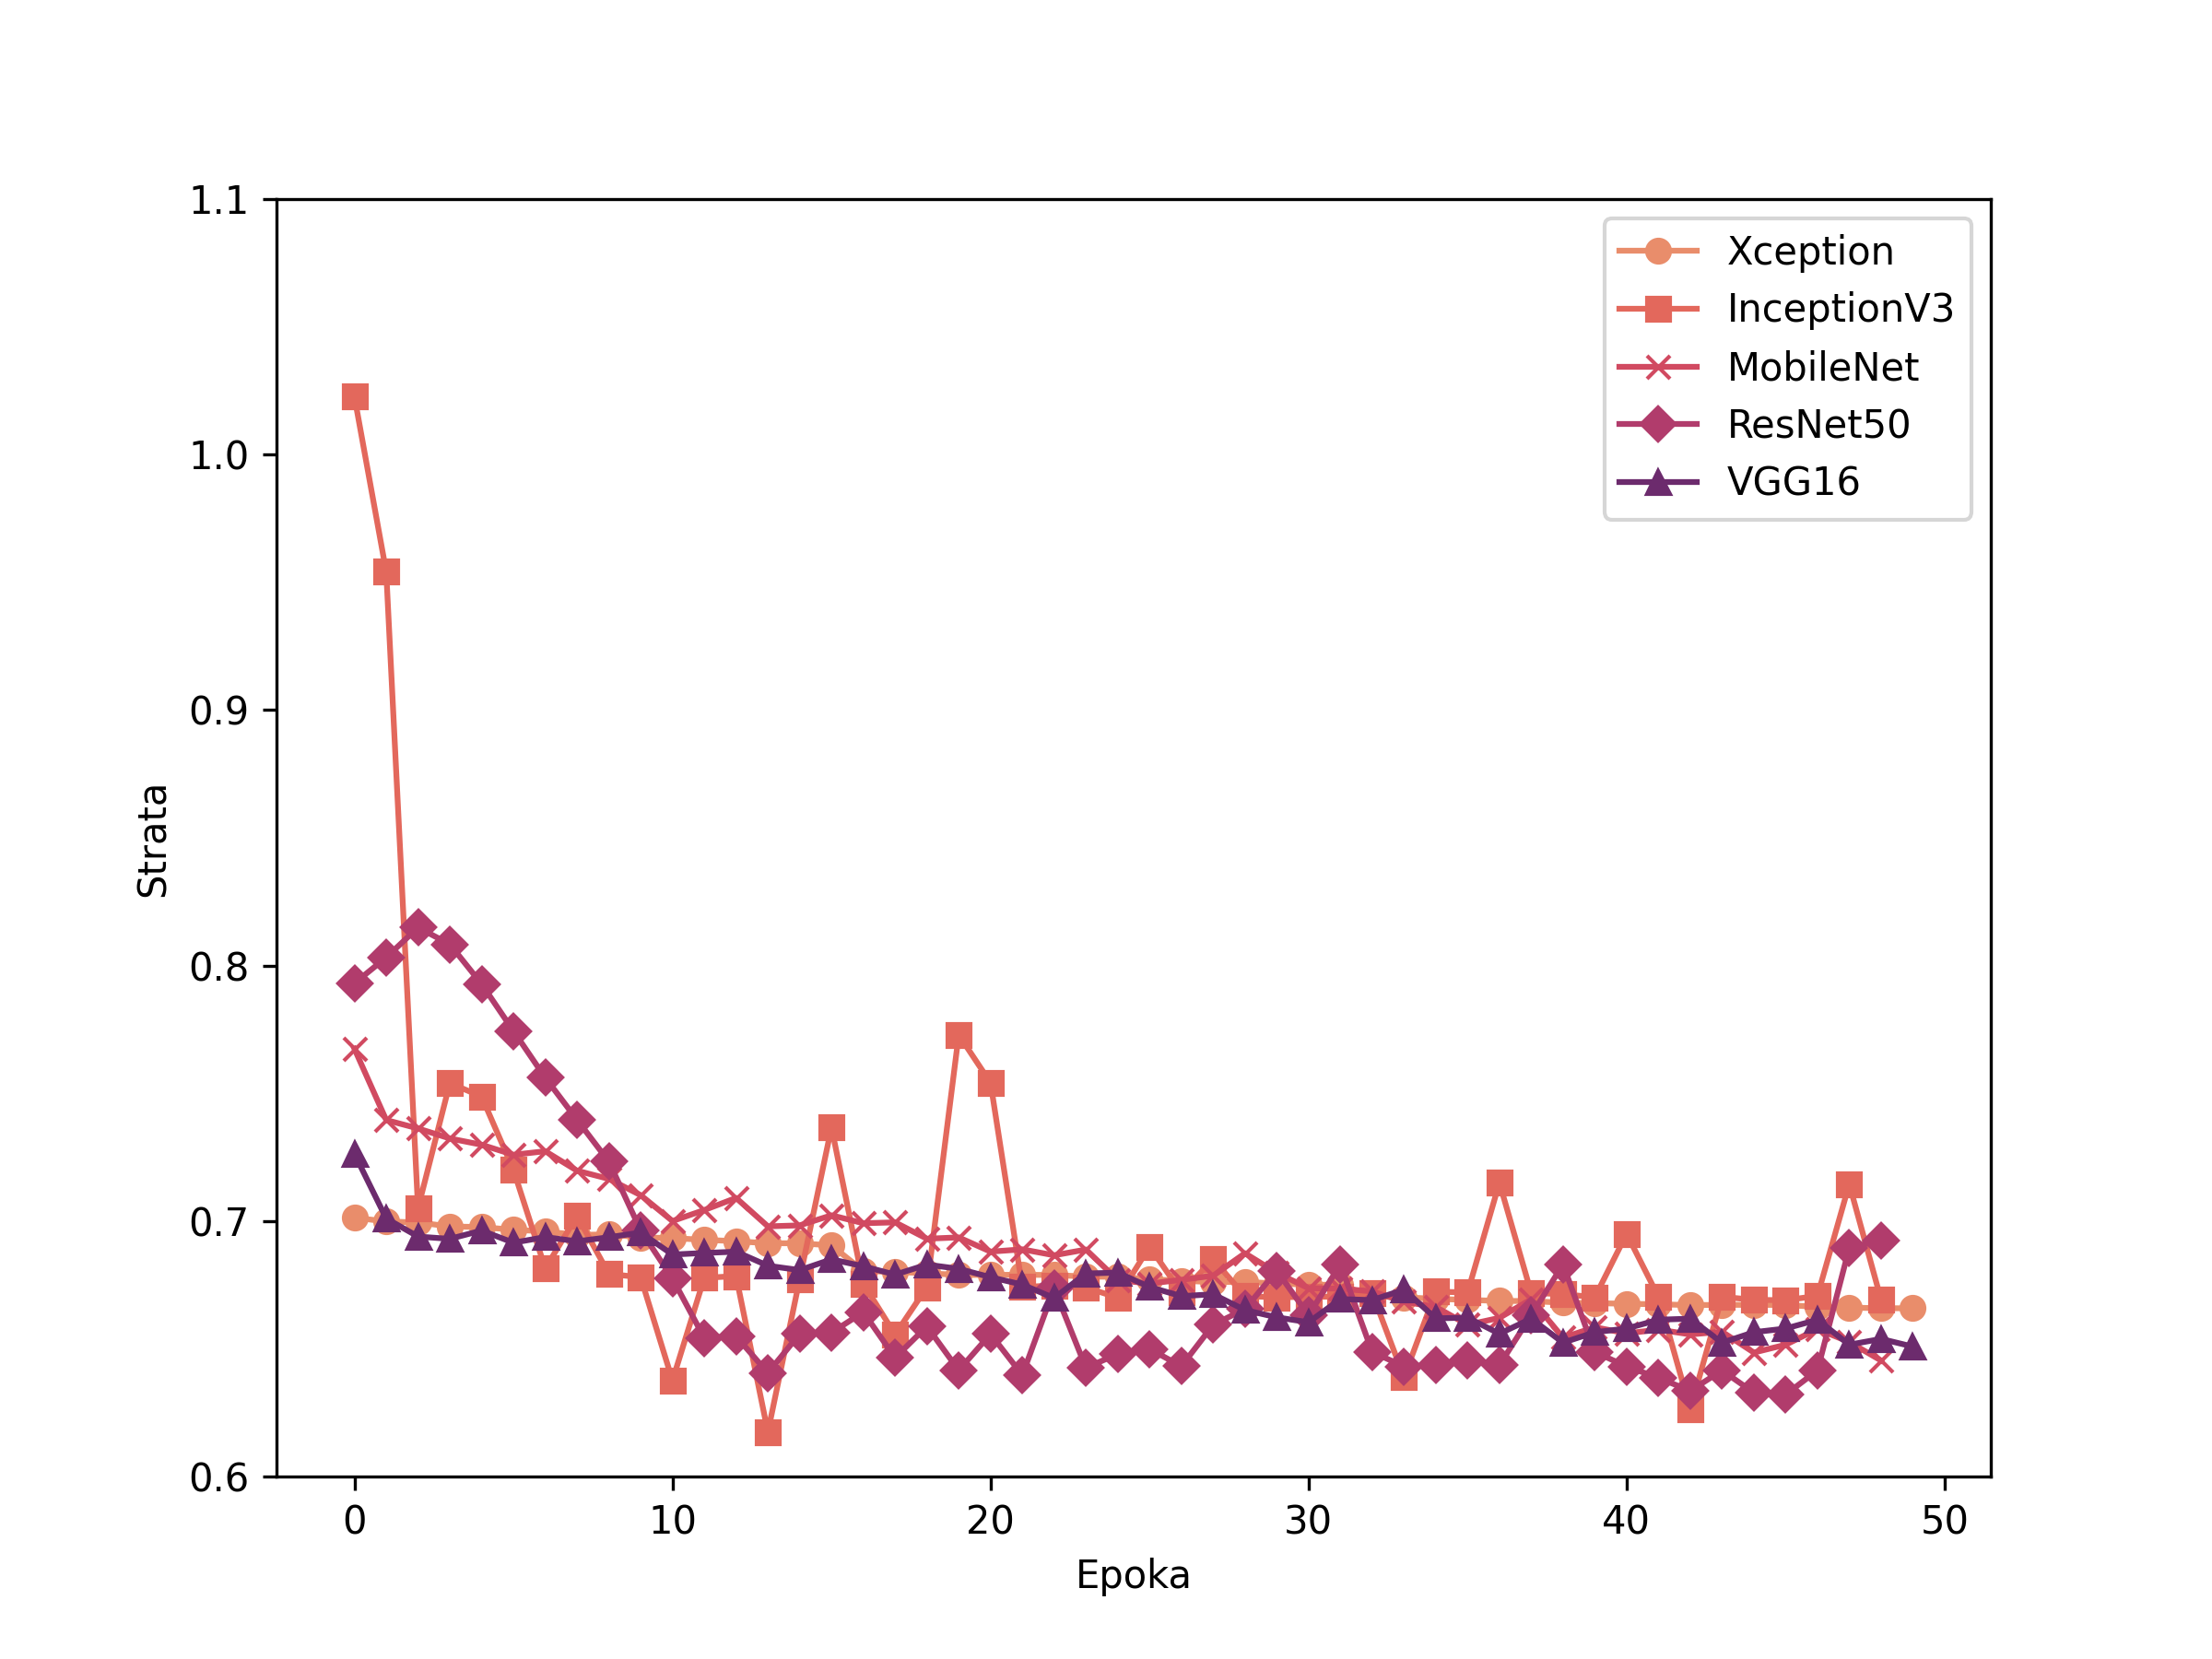
\includegraphics[width=\textwidth]{./img/results/o_loss}
        \caption{Krzywe funkcji straty na zbiorze walidacyjnym podczas uczenia\@}
        \label{fig:o_loss}
    \end{subfigure}

    \caption{Porównanie krzywych uczenia dla różnych klasyfikatorów na zbiorze walidacyjnym (samogłoska /o/)}
    \label{fig:o_results}
\end{figure}
%---------------------------------------------------------------------------

\section{Samogłoska /u/}
\label{sec:samogloska-u}

\begin{table}[h]
\centering
\caption{Wyniki otrzymane dla samogłoski /u/}
\label{tab:wyniki-u}
\begin{tabular}{|l|c|c|c|c|c|}
\hline
\textbf{Model} &\textbf{VGG16} &\textbf{Resnet50} &\textbf{Xception} &\textbf{InceptionV3} &\textbf{MobileNetV2} \\ \hline
    Accuracy &0.724 &0.642 &0.663 &0.705 &0.642 \\ \hline
    Precision &0.730 &0.689 &0.682 &0.714 &0.686 \\ \hline
    Recall &0.715 &0.636 &0.657 &0.709 &0.635 \\ \hline
    F1-score &0.712 &0.615 &0.657 &0.708 &0.610 \\ \hline
    Loss &0.654 &0.685 &0.665 &0.637 &0.750 \\ \hline
\end{tabular}
\end{table}

\begin{figure}[ht]
    \centering
    \begin{subfigure}{0.49\textwidth}
        \centering
        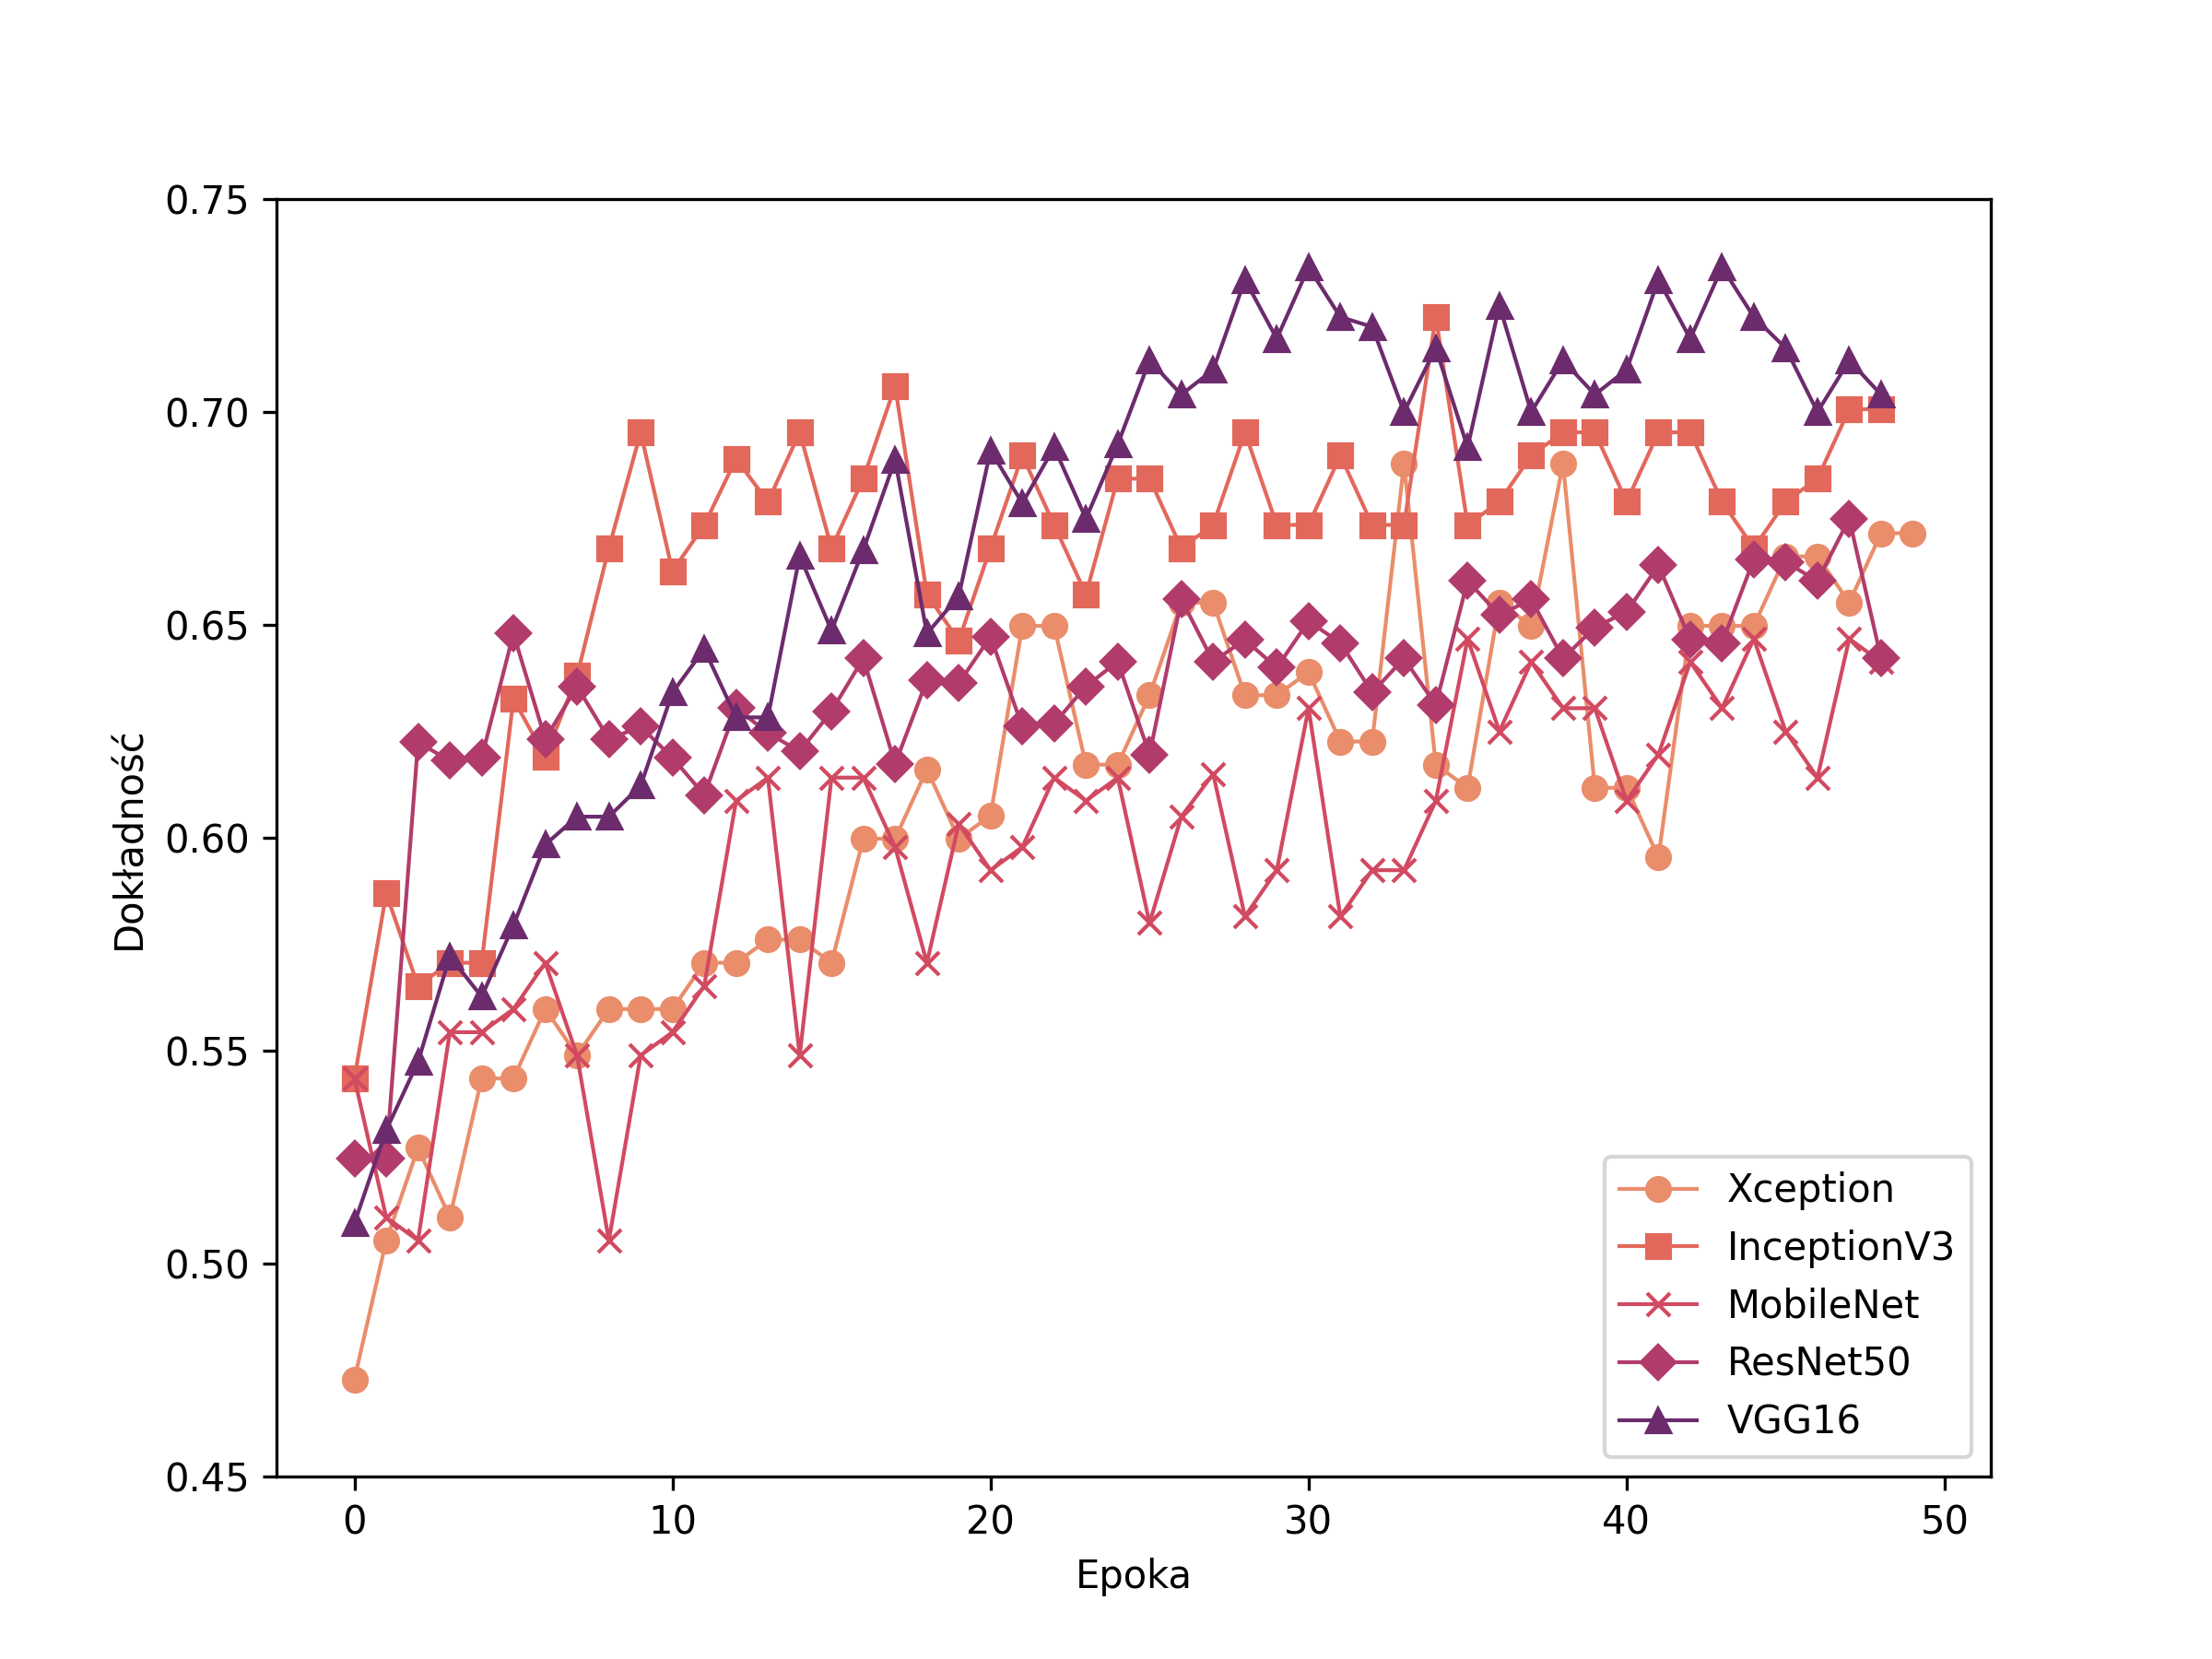
\includegraphics[width=\textwidth]{./img/results/u_acc}
        \caption{Krzywe dokładności na zbiorze walidacyjnym podczas uczenia\@}
        \label{fig:u_acc}
    \end{subfigure}
    \begin{subfigure}{0.49\textwidth}
        \centering
        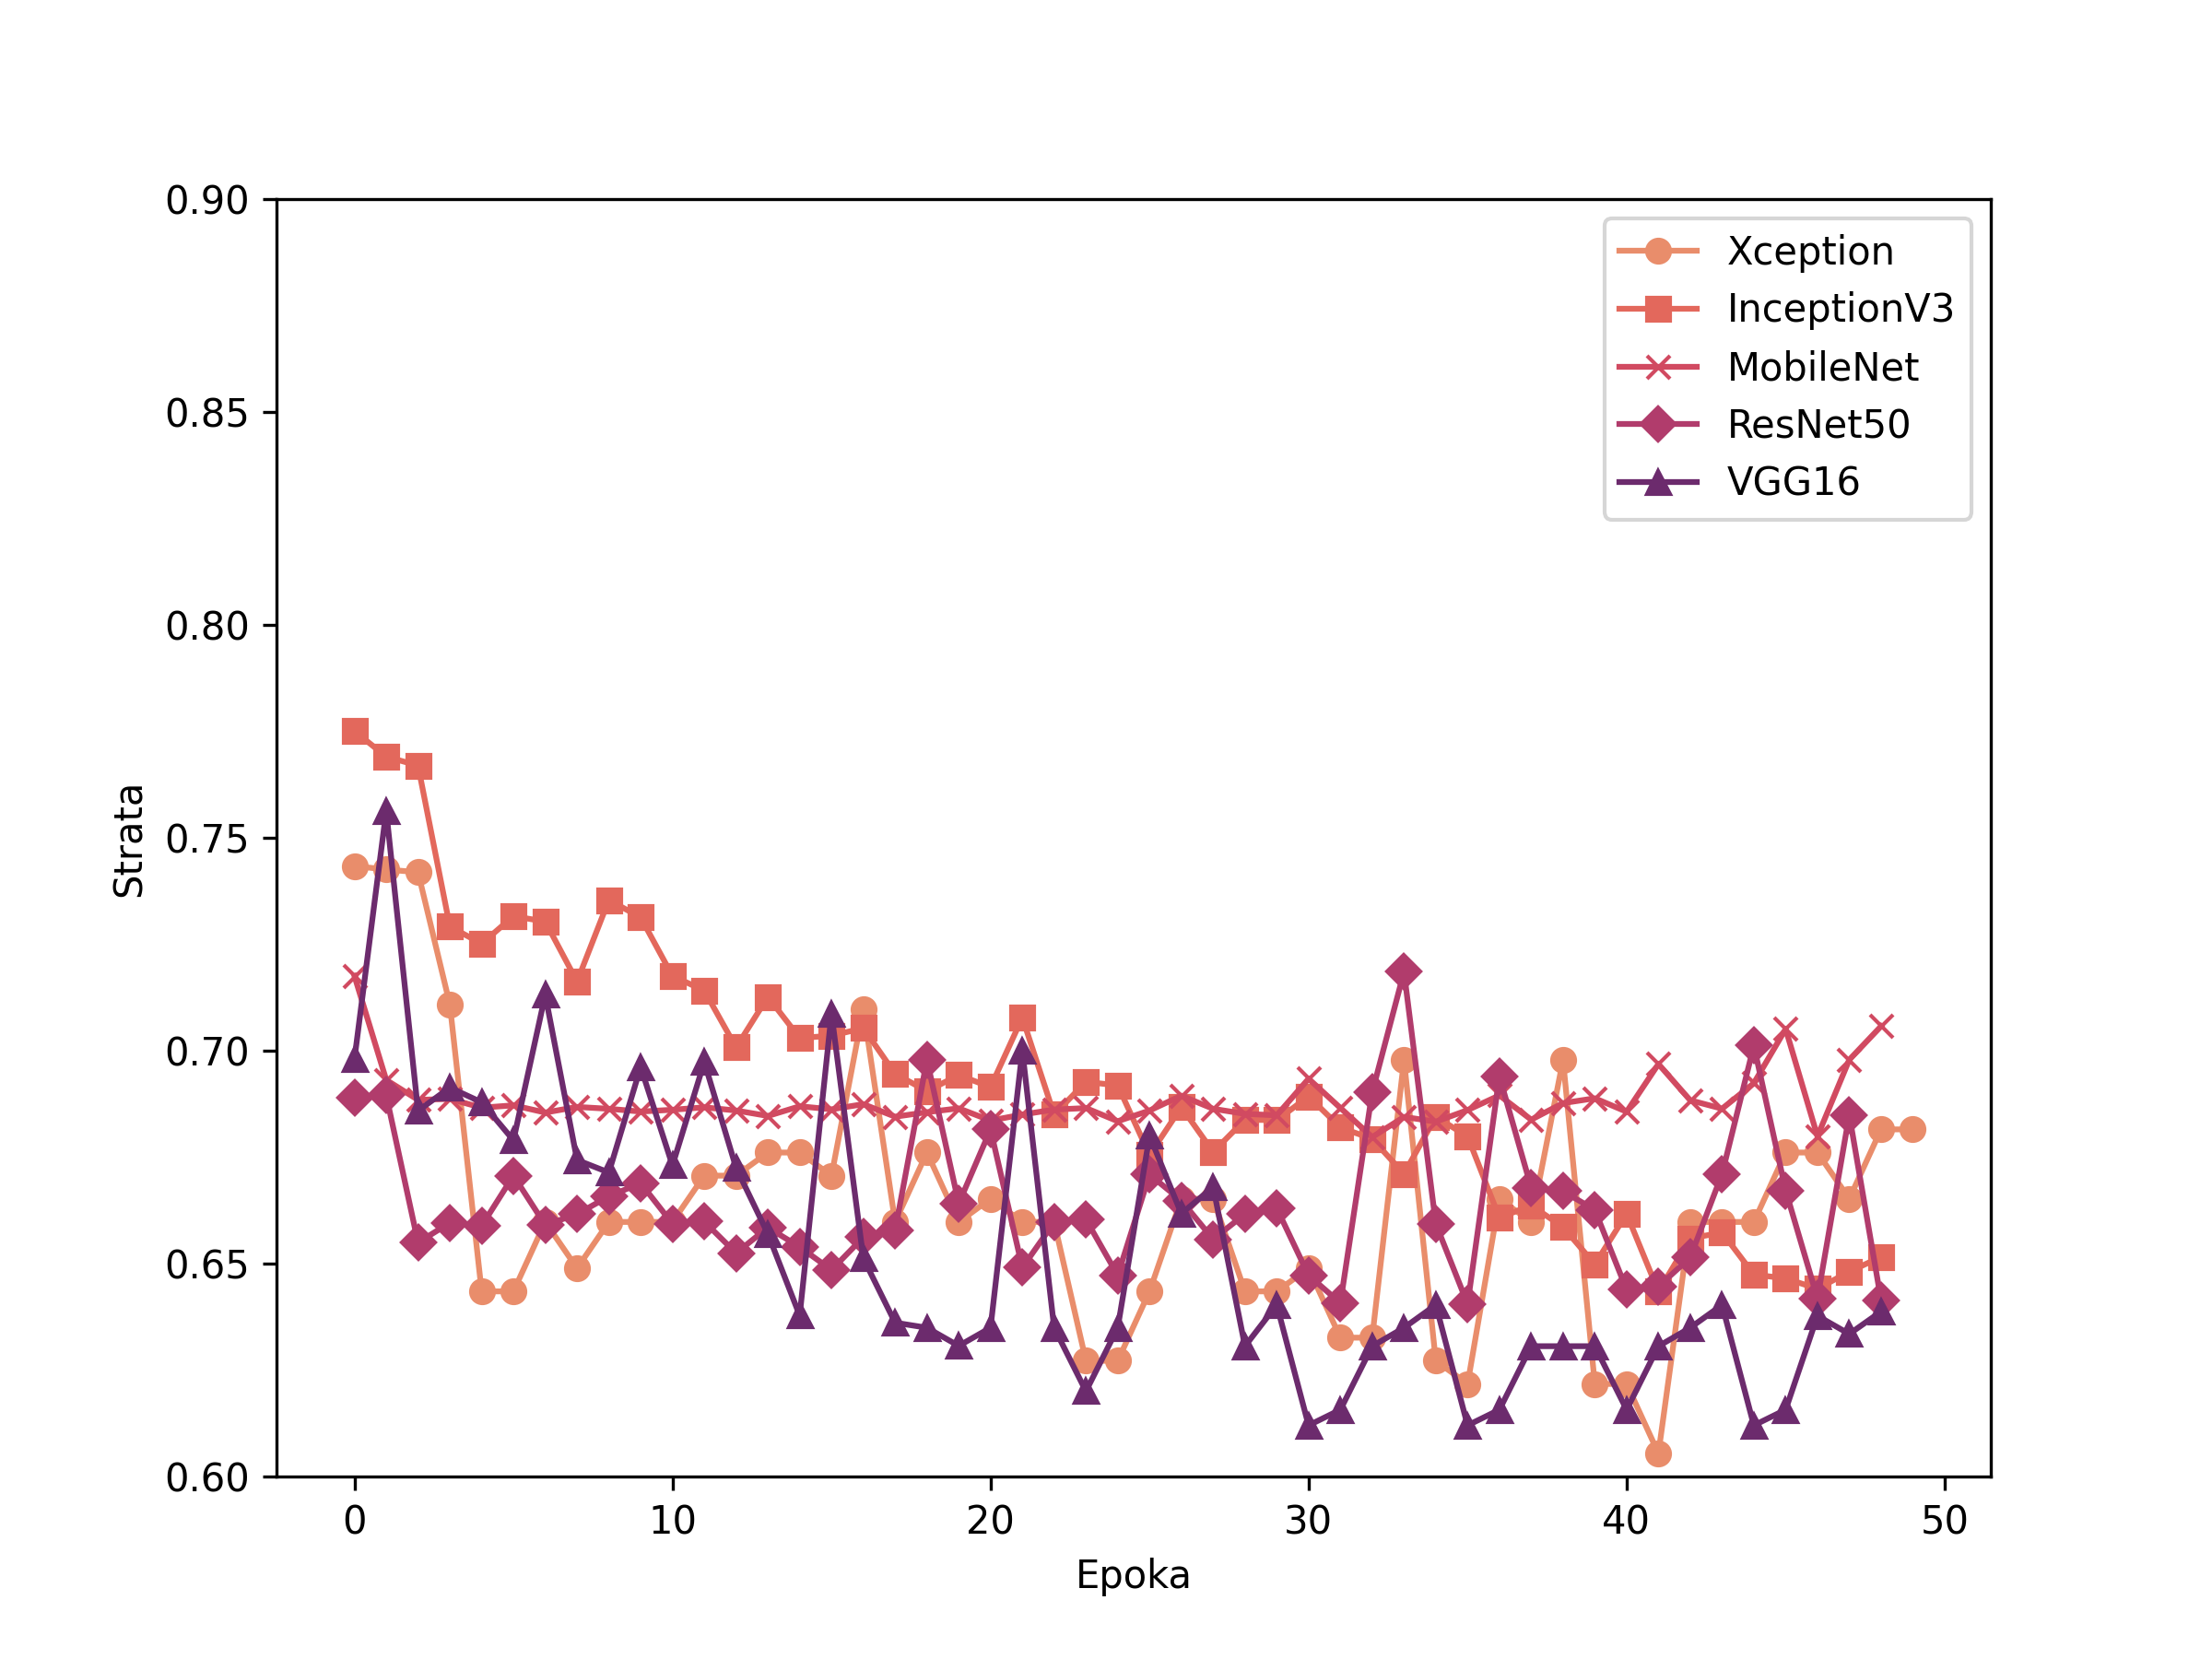
\includegraphics[width=\textwidth]{./img/results/u_loss}
        \caption{Krzywe funkcji straty na zbiorze walidacyjnym podczas uczenia\@}
        \label{fig:u_loss}
    \end{subfigure}

    \caption{Porównanie krzywych uczenia dla różnych klasyfikatorów na zbiorze walidacyjnym (samogłoska /u/)}
    \label{fig:u_results}
\end{figure}
%---------------------------------------------------------------------------
\section{Połączenie samogłosek /a/, /e/, /i/, /o/, /u/}
\label{sec:samogloski}

%---------------------------------------------------------------------------

\section{Zbiorcze podsumowanie wyników}
\label{sec:podsumowanie-wynikow}